\chapter[Compressible Navier-Stokes for Reacting Flows]{\label{chap:fin-s}The Thermochemical Nonequilibrium Compressible Navier-Stokes Equations \\ \vspace{1em} \huge{\textit{Fully-Implicit Navier-Stokes (FIN-S)}}}

%%%%%%%%%%%%%%%%%%%%%%%%%%%%%%%%%%%%%%%%%%%%%%%%%%%%%%%%%%%%%%%%%%%%%%%%%%%%%%%
%%%%%%%%%%%%%%%%%%%%%%%%%%%%%%%%%%%%%%%%%%%%%%%%%%%%%%%%%%%%%%%%%%%%%%%%%%%%%%%
At hypersonic speeds, atmospheric cruise and entry vehicles experience effects which depart considerably from the familiar calorically perfect gas regime.  At flight speeds above Mach~5, the nitrogen and oxygen molecules become vibrationally excited, and the gas becomes thermally perfect.  As the freestream Mach number is increased further, molecular oxygen begins to dissociate.  The resulting atomic oxygen is then free to react with the molecular nitrogen, and nitric oxide may be formed.  At still higher speeds (in excess of Mach 15) the nitrogen molecules begin to dissociate.  At speeds above Mach 25 the gas becomes weakly ionized~\cite{anderson_hypersonic}.

When the time scale associated with chemical reactions in the flow is much less than the fluid dynamic time scales, $t_{\text{chem}} \ll t_{\text{flow}}$, the gas can be assumed to be in equilibrium.  In this situation the equilibrium principle holds and the state of the gas is uniquely determined by any two independent thermodynamic properties.  Conversely, when the time scale associated with chemical reactions is much greater than the fluid dynamic time scales, $t_{\text{chem}} \gg t_{\text{flow}}$, the gas is said to be frozen.  In this case the chemical composition of the gas is fixed throughout the domain, and the fluid may be adequately modeled as a nonreacting mixture of thermally perfect gases.

Between these two extremes is the regime of chemical nonequilibrium.  In this case chemical and fluid dynamic time scales are comparable.  The chemical composition at any point in the domain is then not only a function of local conditions, but also of the streamline history.  Conceptually, the gas will begin to adjust to reach its equilibrium state, but before this process has completed it will have convected downstream.  It will then seek a new equilibrium state dictated by the local conditions.  In this situation $t_{\text{chem}}\approx t_{\text{flow}}$, and the chemical composition of the gas itself must be determined.  In this regime the flow is said to be in \emph{chemical nonequilibrium}. For applications of interest in aerospace engineering, these flows can be modeled to good approximation by a chemically reacting mixture of perfect gases.  Note this approach assumes that intermolecular forces are negligible and hence each chemical species in the flow obeys the perfect gas law, an assumption which is generally valid, except for very high pressures at low temperature~\cite{anderson_hypersonic}.

Considering a diatomic molecule, shown schematically in Figure~\ref{fig:notional_diatomic}. It is clear that there are four possible \emph{modes} in which the molecule may store energy  These are:
\begin{figure}[hbtp]
  \begin{center}
    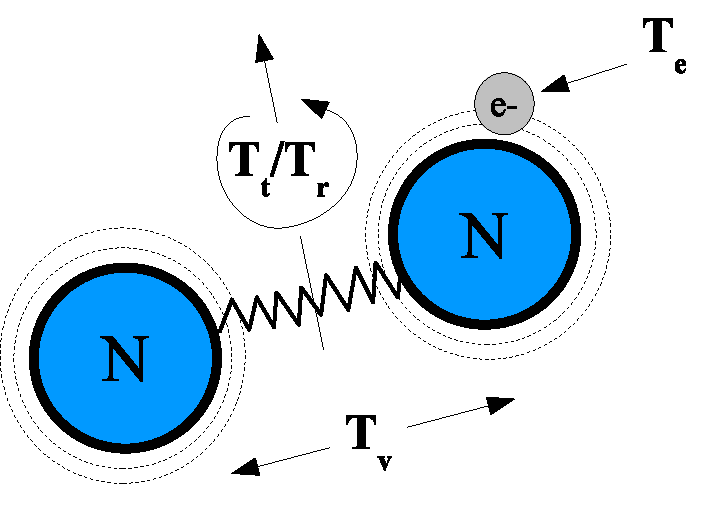
\includegraphics[width=.7\textwidth]{figures/misc/N2}
    \caption{Notional diatomic molecule.\label{fig:notional_diatomic}}
  \end{center}
\end{figure}
\begin{enumerate}
  \item Translational energy due to random motion,
  \item Rotational energy due to rotation about its center of mass,
  \item Vibrational energy due to relative motion between the atoms, and
  \item Electronic energy due to the state of the electrons.
\end{enumerate}
When the molecule is in thermal equilibrium, each of these four modes are in equilibrium with each other, and all modes can adequately be described by a single temperature $T$.  When the gas is not in thermal equilibrium, however, each energy mode is potentially distinct and must be characterized by its own temperature, $T_t, T_r, T_v, T_e$.  Further, each molecular species in the gas may be characterized by its own vibrational temperature~\cite{candler_thesis}.

The mechanism by which the energy modes are equilibrated is through collisions.  It is traditionally assumed that the translational and rotational modes equilibrate very rapidly (within $\mathcal{O}(5-10)$ collisions~\cite{candler_thesis,lordi_mates_rotational_relaxation}), therefore they may modeled with a single translational/rotational temperature $T\equiv T_t=T_r$. It is worth noting that recent research may refute this assumption for the case of nitrogen passing through a very strong shock~\cite{park_N2_rotational_relaxation}, suggesting that this assumption may need to be revisited in the future.

By contrast, the vibrational modes require many more collisions to equilibrate.  As in the case of chemical nonequilibrium, it is entirely possible that during the process of vibrational equilibration the gas will convect downstream to a point in the flow with a different equilibrium vibrational state~\cite{anderson_hypersonic}.  In this situation we must consider the vibrational energy as separate and distinct from the translational/rotational modes.  One common assumption, which we adopt here, is to model the vibrational and electronic temperatures with the same temperature $T_V\equiv T_v=T_e$~\cite{gnoffo_conservation_laws}.  We thus arrive at a two-temperature system for the case of thermal nonequilibrium where $\left(T,T_V\right)$ 

The remainder of this paper is outlined as follows.  Section~\ref{sec:comp_ns_math_model} reviews the compressible Navier-Stokes equations for a reacting mixture of perfect gases in thermal nonequilibrium. Section~\ref{sec:comp_ns_weak} then presents the stabilized weak form of the governing equations and describes the associated finite element discretization.  The finite element formulation is then presented in Section~\ref{sect:comp_fe_formulation}.  The parallel solution methodology is briefly  described in Section~\ref{sec:comp_solution_methodology}, and the performance of the algorithm is then investigated with numerical experiments and validation cases in Section~\ref{chap:compressible:applications}.  Finally, some general observations are drawn and areas for future research are discussed in Section~\ref{sec:conclusions}


%%%%%%%%%%%%%%%%%%%%%%%%%%%%%%%%%%%%%%%%%%%%%%%%%%%%%%%%%%%%%%%%%%%%%%%%%%%%%%%
%%%%%%%%%%%%%%%%%%%%%%%%%%%%%%%%%%%%%%%%%%%%%%%%%%%%%%%%%%%%%%%%%%%%%%%%%%%%%%%
\section{Mathematical Model\label{sec:comp_ns_math_model}}
The compressible Navier--Stokes equations describe the conservation of mass, momentum, and energy for this class of flows.  This section summarizes the Navier--Stokes system of equations, relevant state equations and transport property models for non-ionized air in thermochemical nonequilibrium.

%%%%%%%%%%%%%%%%%%%%%%%%%%%%%%%%%%%%%%%%%%%%%%%%%%%%%%%%%%%%%%%%%%%%%%%%%%%%%%%
\subsection{Conservation Equations}
The conservation of mass, momentum, and total energy for a compressible fluid composed of $ns$ constitutive components may be written as
\begin{align}
  \label{eq:pde_comp_mass_us}
  \pdv{\rho_s}{t} &+ \grad{}\cdot \rho_s\left(\bv{u} + \bv{u}_s\right) = \dot{\omega}_s \\
  \label{eq:pde_comp_mom_us}
  \pdv{\rho\bv{u}}{t} &+ \grad{}\cdot\left(\rho\bv{u}\bv{u}\right) =
    -\grad{P} + \grad{}\cdot\bt{\tau} \\
  \label{eq:pde_comp_energy_us}
  \pdv{\rho E}{t} &+ \grad{}\cdot\left(\rho\bv{u}H\right) + \grad{}\cdot\left(\sum_{s=1}^{N_s}\rho_s\bv{u}_sh_s \right) =
    -\grad{}\cdot\bv{q}   + \grad{}\cdot\left(\bt{\tau}\bv{u}\right)  
\end{align}
where $\rho_s$ is the density of species $s$, $\rho=\sum_s \rho_s$ is the mixture density, $\bv{u}$ is the mixture velocity, $\bv{u}_s$ is the diffusion velocity of species $s$, $E$ is the total energy per unit mass, and $P$ is the pressure.  The total enthalpy, $H$, may be expressed in terms of the total energy, density, and pressure: $H = E + P/\rho$.  The viscous stress tensor $\bt{\tau}$ and the heat flux vector $\bv{q}$ are defined as
\begin{align}
  \label{eq:stress_tensor}
  \bv{\tau} &= \mu\left(\grad{\bv{u}} + \tgrad{\bv{u}}\right) -\frac{2}{3}\mu \left(\grad{}\cdot\bv{u}\right)\bt{I} \\
  \label{eq:fouriers_law}
  \bv{q} &= -k\grad{T} - k_v\grad{T_v} - k_e\grad{T_e}
\end{align}
where $\mu$ is the dynamic viscosity, $k$ is the thermal conductivity, $T,T_v,T_e$ are respectively the fluid translational/rotational, vibrational, and electron/electronic excitation temperatures, and $\bt{I}$ denotes the identity matrix.  

For flows in which thermal equilibrium holds, the same temperature $T=T_v=T_e$ governs all energy modes.  However, for many applications in hypersonic flows, thermal equilibrium does not exist.  This is because of the relatively large number of collisions required to equilibrate the vibrational energies of molecules.  In general vibrational states require an order of magnitude or more collisions to equilibrate than translational/rotational states.  Recognizing this, a common approach is to assume a \emph{two temperature} model in which the translational/rotational energy is governed by the the temperature, $T$, while the vibrational and electronic energy are governed by a separate temperature $T_V=T_v=T_e$.  In this situation the vibrational/electronic energy are governed by a separate transport equation:
\begin{equation}
  \label{eq:pde_comp_energy_V_us}
  \pdv{\rho e_V}{t} + \grad{}\cdot\left(\rho e_V \bv{u}\right) + \grad{}\cdot\left(\sum_{s=1}^{N_s}\rho_s e_{Vs} \bv{u}_s\right) =
    -\grad{}\cdot\bv{q}_V + \dot{\omega}_V
\end{equation}
For the two-temperature model applied to a non-ionized flow the vibrational heat flux is given by $\bv{q}_V = - k_V\grad{T_V}$.

In general, the species diffusion velocities $\bv{u}_s$ result from gradients in species concentration, temperature, and pressure.  However, for most flows of interest in aerospace applications, only the species concentration term is significant.  We adopt this assumption in this work, therefore species diffusion is driven solely by concentration gradients.  Under this assumption the species diffusion velocities are given by Fick's law as
\begin{equation}
  \label{eq:species_velocities}
  \rho_s \bv{u}_s = -\rho \mathcal{D}_s \grad{c_s}
\end{equation}
where $c_s=\left(\rho_s/\rho\right)$ is the mass fraction of species $s$.  Combining Equations~\eqref{eq:pde_comp_mass_us}--\eqref{eq:pde_comp_energy_V_us} with~\eqref{eq:species_velocities} yields the following set of equations:
\begin{align}
  \label{eq:pde_comp_mass}
  \pdv{\rho_s}{t} &+ \grad{}\cdot \left(\rho_s\bv{u}\right) = \grad{}\cdot\left(\rho \mathcal{D}_s \grad{c_s}\right) + \dot{\omega}_s \\
  \label{eq:pde_comp_mom}
  \pdv{\rho\bv{u}}{t} &+ \grad{}\cdot\left(\rho\bv{u}\bv{u}\right) =
    -\grad{P} + \grad{}\cdot\bt{\tau} \\
  \label{eq:pde_comp_energy}
  \pdv{\rho E}{t} &+ \grad{}\cdot\left(\rho \bv{u} H\right) =
    -\grad{}\cdot\bv{q} + \grad{}\cdot\left(\rho \sum_{s=1}^{N_s} h_s \mathcal{D}_s \grad{c_s}\right)  + \grad{}\cdot\left(\bt{\tau}\bv{u}\right)   \\
  \label{eq:pde_comp_energy_V}
  \pdv{\rho e_V}{t} &+ \grad{}\cdot\left(\rho e_V \bv{u}\right) =
    -\grad{}\cdot\bv{q}_V + \grad{}\cdot\left(\rho \sum_{s=1}^{N_s} e_{Vs} \mathcal{D}_s \grad{c_s}\right)  + \dot{\omega}_V
\end{align}
which describe the viscous flow of a chemically reacting mixture of gases in thermal nonequilibrium.  The special case of thermal equilibrium is recovered simply by omitting the last equation.

\subsubsection{Thermodynamics}

The total energy, $E$, is composed of internal and kinetic components: $E = e^{\text{int}} + \bv{u}\cdot\bv{u}/2$.  In turn, the total internal energy, $e^{\text{int}}$, has contribution from each of the distinct energy \emph{modes}.  Specifically
\begin{align}
  e^{\text{int}} &= e^{\text{trans}} + e^{\text{rot}} + e^{\text{vib}} + e^{\text{elec}}  + h^0 \\
         &= \sum_{s=1}^{N_s} c_s e^{\text{trans}}_s +  \sum_{s=mol} c_s e^{\text{rot}}_s +  \sum_{s=mol} c_s e^{\text{vib}}_s +  \sum_{s=1}^{N_s} c_s e^{\text{elec}}_s +  \sum_{s=1}^{N_s} c_s h^0_s  \label{eq:energy_partition}
\end{align}
The first four terms on the right of Equation~\eqref{eq:energy_partition} represent the energy due to molecular/atomic translation, molecular rotation, molecular vibration, and electronic excitation.  The final term is the heat of formation of the mixture and accounts for the energy stored in chemical bonds.  To good approximation the translational and rotational states of the gas may be assumed fully populated, and under this assumption the translational/rotational energy for each species may be expressed as
\begin{equation}
  \label{eq:e_tr_combined}
  e^{\text{trans}}_s + e^{\text{rot}}_s = e^{\text{tr}}_s = C^{\text{tr}}_{v,s}\, T
\end{equation}
where the translational/rotational specific heat, $C^{\text{tr}}_{v,s}$ is given by
\begin{equation}
  C^{\text{tr}}_{v,s} = 
  \begin{cases}
    \frac{5}{2} R_s & \text{for molecules}, \\
    \frac{3}{2} R_s & \text{for atoms.}
  \end{cases}
\end{equation}
where $R_s$ is the species gas constant, and $R_s = R/M_s$ where $R$ is the universal gas constant and $M_s$ is the species molar mass.  The combined term $e^{\text{tr}}_s$ in Equation~\eqref{eq:e_tr_combined} represents the energy due to random thermal translational/rotational motion of a given species.

In contrast to the translational/rotational states, the vibrational energy states are typically not fully populated. One approach for modeling the molecular vibrational energy is through analogy to a harmonic oscillator.  In this approach the energy potential between molecular nuclei is modeled as a quadratic function of separation distance.  Under this assumption, the vibrational energy for each molecular species can be modeled as
\begin{equation}
  \label{eq:species_vibrational_energy}
  e^{\text{vib}}_s = 
  \begin{cases}    
    0 & \text{for atoms}, \\
    \frac{R_s\theta_{vs}}{\exp\left(\theta_{vs}/T_v\right) - 1} & \text{for diatomic molecules}, \\
    \sum_i \frac{R_s\theta_{vs,i}}{\exp\left(\theta_{vs,i}/T_v\right) - 1} & \text{for general molecules}
  \end{cases}
\end{equation}
where $\theta_{vs}$ is the species characteristic temperature of vibration and $T_v$ is the mixture vibrational temperature.

The energy contained in the excited electronic states for a given species, $e^{\text{elec}}_s$, can be obtained from the assumption that they are in a Boltzmann distribution governed by the electronic excitation temperature $T_e$ as~\cite{candler_thesis}
\begin{equation}
  \label{eq:elec_excitation}
  e^{\text{elec}}_s = R_s \frac{\sum_{i=1}^\infty \theta^{\text{elec}}_{is} g_{is} \exp\left(-\theta^{\text{elec}}_{is}/T_e\right)}{g_{0s} + \sum_{i=1}^\infty g_{is} \exp\left(-\theta^{\text{elec}}_{is}/T_e\right)}
\end{equation}
Recall that for the two-temperature model the vibrational and electronic excitation temperatures are assumed to be identical, that is $T_v=T_e\equiv T_V$, and that in the case of thermal equilibrium $T_r=T_t=T_v=T_e\equiv T$.

In practice, Equation~\eqref{eq:elec_excitation} can usually be omitted for non-ionized flows such as those considered in this work. Park~\cite{park_book} observes that electronic transitions in molecules are caused mostly by the impact of free electrons.  Since there are no free electrons when there is no ionization, there will be very little electronic excitation.  In the present work we choose to retain Equation~\eqref{eq:elec_excitation} for completeness and to aid in future expansion to weakly ionized flows.

Combining the terms above, it is clear that in the case of thermal nonequilibrium
\begin{equation}
  \label{eq:rE-T-Tv-relationship}
  \rho E =  \frac{1}{2}\rho\left(\bv{u}\cdot\bv{u}\right) + \sum_{s=1}^{N_s} \rho_s C^{\text{tr}}_{v,s} T + \rho e_V  + \sum_{s=1}^{N_s} \rho_s h^0_s
\end{equation}
where the term $\rho e_V $ is provided by Equation~\eqref{eq:pde_comp_energy_V}.  Equation~\eqref{eq:rE-T-Tv-relationship} is linear in $T$ and therefore may be inverted directly to find the translational/rotational temperature $T$, however the vibrational/electronic temperature  $T_V$ must be computed iteratively from the relation
\begin{equation}
  \label{eq:rev-Tv-relationship}
  \rho e_V\left(T_V\right) = \sum_{s=mol} \rho_s e^{\text{vib}}_s\left(T_V\right) + \sum_{s=1}^{N_s} \rho_s e^{\text{elec}}_s\left(T_V\right)
\end{equation}
In the case of thermal equilibrium we have 
\begin{equation}
  \label{eq:rE-T-relationship}
  \rho E =  \frac{1}{2}\rho\left(\bv{u}\cdot\bv{u}\right) + \sum_{s=1}^{N_s} \rho_s C^{\text{tr}}_{v,s} T + \sum_{s=mol} \rho_s e^{\text{vib}}_s\left(T\right) + \sum_{s=1}^{N_s} \rho_s e^{\text{elec}}_s\left(T\right) + \sum_{s=1}^{N_s} \rho_s h^0_s
\end{equation}
which is clearly nonlinear in the equilibrium temperature $T$.  In practice, a Newton iteration is performed to determine $T$ or $T_V$ from Equations~\eqref{eq:rev-Tv-relationship}--\eqref{eq:rE-T-relationship} as required, and this procedure typically converges in 2-3 iterations.  

Regardless of the thermal state of the mixture, once the translational/rotational temperature $T$ is determined the thermodynamic pressure of the mixture is readily obtained from Dalton's law of partial pressures:
\begin{equation}
  P = \sum_{s=1}^{N_s}  P_s = \sum_{s=1}^{N_s} \rho_s R_s T 
  \label{eq:p_eq_state}
\end{equation}

Because of the nonlinearity of vibrational and electronic energies,
the corresponding specific heats in these cases are not constant, but
are defined only through derivatives of the above energy equations:
\begin{align}
C^{\text{vib}}_{v,s} &= \pdv{e^{\text{vib}}_{v,s}}{T_V} \\
C^{\text{elec}}_{v,s} &= \pdv{e^{\text{elec}}_{v,s}}{T_V}
\end{align}
with the vibrational energy $e^{\text{vib}}_{v,s}$ from
Equation~\eqref{eq:species_vibrational_energy} and the 
electronic energy $e^{\text{elec}}_{v,s}$ given by
Equation~\eqref{eq:elec_excitation}.
%
Combined terms $C^{\text{ve}}_{v,s}$ or $C_{v,s}$ can be defined as
\begin{align}
  C^{\text{ve}}_{v,s} &= C^{\text{vib}}_{v,s} + C^{\text{elec}}_{v,s} \\
  C_{v,s} &= C^{\text{tr}}_{v,s} + C^{\text{ve}}_{v,s}
\end{align}
%
and mixture specific heats are given as
\begin{align}
  C^{\text{vib}}_{v} &= \sum_s c_s
    C^{\text{vib}}_{v,s} \\
  C^{\text{elec}}_{v} &= \sum_s c_s
    C^{\text{elec}}_{v,s} \\
  C^{\text{ve}}_{v} &=  \sum_s c_s
    C^{\text{ve}}_{v,s} \\
  C^{\text{tr}}_{v} &= \sum_s c_s
    C^{\text{tr}}_{v,s} \\
  C_{v} &= \sum_s c_s
    C_{v,s}
\end{align}

These are specific heats at constant volume; specific heat at constant
pressure is given as
\begin{equation}
C_p = C_v + R
\end{equation}

\subsection{Chemical Kinetics}
The rate of production/destruction of the individual species, $\dot{\omega}_s$, is required to close the species continuity equations.  To develop these relationships it is instructive to consider the case of a specific mixture.  To this end, let us consider the chemical reactions which occur among the principal components of dissociating air: $\text{N}_2,\text{O}_2,\text{NO},\text{N},\text{O}$.  For this mixture the primary chemical reactions that occur are
\begin{align*}
  \text{N}_2 + \mathcal{M} &\rightleftharpoons 2\text{N} + \mathcal{M} \\
  \text{O}_2 + \mathcal{M} &\rightleftharpoons 2\text{O} + \mathcal{M} \\
  \text{NO} + \mathcal{M}  &\rightleftharpoons \text{N} + \text{O} + \mathcal{M} \\
  \text{N}_2 + \text{O}    &\rightleftharpoons \text{NO} + \text{N} \\
  \text{NO} + \text{O}     &\rightleftharpoons \text{O}_2 + \text{N}  
\end{align*}
These reactions can occur in either the forward or backward direction, as denoted by the bidirectional arrows.  The reactions are presented such that they are endothermic in the forward direction~\cite{wright_thesis}.  In these reactions $\mathcal{M}$ denotes a generic collision partner, which may be any of the species present in the flow. In the case of dissociation, the collision partner provides the energy required to break the molecular bond.  By contrast, during recombination the collision partner absorbs the dissociation energy from the atomic pair.  The collision partner is otherwise unaltered by the reaction.

Each of the $r$ reactions is governed by a forward and backward rate coefficient, $k_{fr}$ and $k_{br}$.  The rate of each reaction is therefore a sum of the forward and backward rates:
\begin{align*}
  \mathcal{R}_1 &= \sum_{m\in\mathcal{M}}\left(k_{b1m}\frac{\rho_{\text{N}}}{M_{\text{N}}}\frac{\rho_{\text{N}}}{M_{\text{N}}}\frac{\rho_{\text{m}}}{M_{\text{m}}} - k_{f1m}\frac{\rho_{\text{N}_2}}{M_{\text{N}_2}}\frac{\rho_{\text{m}}}{M_{\text{m}}} \right) \\  
  \mathcal{R}_2 &= \sum_{m\in\mathcal{M}}\left(k_{b2m}\frac{\rho_{\text{O}}}{M_{\text{O}}}\frac{\rho_{\text{O}}}{M_{\text{O}}}\frac{\rho_{\text{m}}}{M_{\text{m}}} - k_{f2m}\frac{\rho_{\text{O}_2}}{M_{\text{O}_2}}\frac{\rho_{\text{m}}}{M_{\text{m}}} \right) \\
  \mathcal{R}_3 &= \sum_{m\in\mathcal{M}}\left(k_{b3m}\frac{\rho_{\text{N}}}{M_{\text{N}}}\frac{\rho_{\text{O}}}{M_{\text{O}}}\frac{\rho_{\text{m}}}{M_{\text{m}}} - k_{f3m}\frac{\rho_{\text{NO}}}{M_{\text{NO}}}\frac{\rho_{\text{m}}}{M_{\text{m}}} \right) \\
  \mathcal{R}_4 &= k_{b4}\frac{\rho_{\text{NO}}}{M_{\text{NO}}}\frac{\rho_{\text{N}}}{M_{\text{N}}} - k_{f4}\frac{\rho_{\text{N}_2}}{M_{\text{N}_2}}\frac{\rho_{\text{O}}}{M_{\text{O}}} \\
  \mathcal{R}_5 &= k_{b5}\frac{\rho_{\text{O}_2}}{M_{\text{O}_2}}\frac{\rho_{\text{N}}}{M_{\text{N}}} - k_{f5}\frac{\rho_{\text{NO}}}{M_{\text{NO}}}\frac{\rho_{\text{O}}}{M_{\text{O}}}
\end{align*}
Note that each of these $r$ reactions is of the canonical form
\begin{align}
  \mathcal{R}_r &=  \mathcal{R}_{br} - \mathcal{R}_{fr} \\
                &= k_{br} \prod_{s=1}^{N_s} \left(\frac{\rho_s}{M_s}\right)^{\beta_{sr}} - k_{fr} \prod_{s=1}^{N_s} \left(\frac{\rho_s}{M_s}\right)^{\alpha_{sr}}
\end{align}
where $\alpha_{sr}$ and $\beta_{sr}$ are the stoichiometric coefficients for reactants and products of species $s$.

The species source terms can now be expressed in terms of the individual reaction rates as follows
\begin{align*}
  \dot{\omega}_{\text{N}_2} &= M_{\text{N}_2}\left(\mathcal{R}_1 + \mathcal{R}_4\right) \\
  \dot{\omega}_{\text{O}_2} &= M_{\text{O}_2}\left(\mathcal{R}_2 - \mathcal{R}_5\right) \\
  \dot{\omega}_{\text{NO}} &= M_{\text{NO}}\left(\mathcal{R}_3 -\mathcal{R}_4 + \mathcal{R}_5\right) \\
  \dot{\omega}_{\text{N}}  &= M_{\text{N}}\left(-2\mathcal{R}_1 -\mathcal{R}_3 - \mathcal{R}_4 - \mathcal{R}_5\right) \\
  \dot{\omega}_{\text{O}}  &= M_{\text{O}}\left(-2\mathcal{R}_2 -\mathcal{R}_3 + \mathcal{R}_4 + \mathcal{R}_5\right)
\end{align*}
These source terms sum identically to zero, as required by conservation of mass. The source terms are of the canonical form
\begin{equation}
  \dot{\omega}_s = M_s \sum_{r=1}^{nr}\left(\beta_{sr}-\alpha_{sr}\right)\left(\mathcal{R}_{fr} - \mathcal{R}_{br}\right)
\end{equation}
where $nr$ is the number of reactions. 

It remains to determine the rate coefficients $k_{f}$ and $k_{b}$.  To this end, let us first introduce an effective temperature, $\bar{T}$, which is some yet-to-be-specified function of the translational/rotational and vibrational temperatures.  The forward rate coefficients can then be expressed in a modified Arrhenius form as
\begin{equation}
  k_{fr}\left(\bar{T}\right) = C_{fr} \bar{T}^{\eta_r} \exp \left(-E_{ar}/R\bar{T}\right)
\end{equation}
where $C_{fr}$ is the reaction rate constant, $\eta_r$ is the so-called pre-exponential factor, and $E_{ar}$ is the activation energy.  These three constants are determined from curve fits to experimental data.  The corresponding backward rate coefficient can be found using the principle of detailed balance, which states
\begin{equation}
  K_{eq} = \frac{k_{fr}\left(\bar{T}\right)}{k_{br}\left(\bar{T}\right)}
\end{equation}
where $K_{eq}$ is the equilibrium constant and may be obtained either by curve fits or through Gibbs' free energy techniques. Specifically, for reaction $r$ we have

\begin{equation}
  K_{eq,r}\left(T\right) = \left(\frac{P_0}{RT}\right)^{\nu_r}\exp\left[-\sum_s\left(\beta_{sr}-\alpha_{sr}\right)\left(\frac{H^\circ_s}{RT} - \frac{S^\circ_s}{R}\right)\right]
\end{equation}
where
\begin{equation}
  \nu_r \equiv \sum_s\left(\beta_{sr}-\alpha_{sr}\right)
\end{equation}
and the normalized entalpy and entropy data are available from curve fit data~\cite{barnhardt_thesis}.

\subsection{Vibrational/Electronic Energy Production \& Vibrational Relaxation}
For the case of thermal nonequilibrium it remains to define the vibrational/electronic energy source term, $\dot{\omega}_V$, which appears in Equation~\eqref{eq:pde_comp_energy_V}.  This term represents the production/destruction of vibrational/electronic energy in the gas, and is due to (i) the creation of molecules with some vibrational/electronic energy and (ii) the transfer of energy between the various modes in the gas.  That is, 
\begin{equation}
  \dot{\omega}_v = \dot{Q}_{v} + \dot{Q}_{\text{transfer}}
\end{equation}
When molecular species are created in the gas at rate $\dot{\omega}_s$, they contribute vibrational/electronic energy at the rate 
\begin{equation*}
  \dot{Q}_{vs}=\dot{\omega}_s\left(e^{\text{vib}}_{s} + e^{\text{elec}}_{s}\right)
\end{equation*}
so the net vibrational energy production rate is then simply
\begin{equation}
  \label{eq:vibrational_energy_production}
  \dot{Q}_{v} = \sum_{s=1}^{N_s} \dot{\omega}_s\left(e^{\text{vib}}_{s} + e^{\text{elec}}_{s}\right)
\end{equation}

There is also energy transfer among the various energy modes in the gas.  Strictly speaking, one such energy transfer is vibration-vibration coupling between the various molecules in the gas.  However, implicit in the use of a single vibrational energy equation is the assumption that the molecular vibrational energies equilibrate very rapidly and thus are adequately characterized with a single vibrational temperature $T_V$.  There is also energy transfer between translational and vibrational modes as well as rotational and vibrational modes.  These latter two exchanges are grouped together and represented as a single vibrational energy transfer rate $\dot{Q}^{\text{tr-vib}}$.  

In this work we adopt the Landau-Teller model.  In this model the vibrational energy transfer for a given species is
\begin{equation}
  \label{eq:landau_teller_energy_exchange}
  \dot{Q}^{\text{tr-vib}}_s = \rho_s \frac{\hat{e}^{\text{vib}}_{s} - e^{\text{vib}}_s}{\tau^{\text{vib}}_s}
\end{equation}
where $\hat{e}^{\text{vib}}_{s}$ is the species equilibrium vibrational energy (Equation~\eqref{eq:species_vibrational_energy} evaluated at temperature $T$) and the vibrational relaxation time $\tau^{\text{vib}}_s$ is given by Millikan and White
\begin{equation}
  \tau^{\text{vib}}_s = \frac{\sum_{r=1}^{N_s} \chi_r}{\sum_{r=1}^{N_s} \chi_r/\tau^{\text{vib}}_{sr}}
\end{equation}
where $\chi_r$ is given by
\begin{equation}
  \label{eq:chi_definition}
  \chi_r = c_r\frac{M}{M_r},\;\; M=\left(\sum_{s=1}^{N_s}\frac{c_s}{M_s}\right)^{-1}
\end{equation}
and
\begin{align}
  \label{eq:tau_vib_sr}
  \tau^{\text{vib}}_{sr} &=  \frac{1}{P} \exp\left[A_{sr}\left(T^{-1/3} - 0.015 \mu^{1/4}_{sr}\right) - 18.42\right] \\
          A_{sr} &= 1.16\times 10^{-3} \mu^{1/2}_{sr}\theta_{vs}^{4/3} \\
        \mu_{sr} &= \frac{M_s M_r}{M_s + M_r}
\end{align}
where the pressure in Equation~\eqref{eq:tau_vib_sr} is in units of atmospheres. Combining~\eqref{eq:landau_teller_energy_exchange} and~\eqref{eq:vibrational_energy_production} yields the desired net vibrational energy source term
\begin{equation}
  \dot{\omega}_V = \sum_{s=1}^{N_s} \dot{Q}^{\text{tr-vib}}_s + \sum_{s=1}^{N_s} \dot{\omega}_s\left(e^{\text{vib}}_{s} + e^{\text{elec}}_{s}\right)
\end{equation}


%%%%%%%%%%%%%%%%%%%%%%%%%%%%%%%%%%%%%%%%%%%%%%%%%%%%%%%%%%%%%%%%%%%%%%%%%%%%%%%
\subsection{Transport Properties}
\subsubsection{Single-Species Flows at Low Temperatures}
For flows of a single constituent species at low to moderate temperatures the dynamic viscosity can be computed via Sutherland's law, which is of the form
\begin{equation}
  \mu\left(T\right) = \mu_{\text{ref}} \frac{T^{3/2}}{T + T_{\text{ref}}}
\end{equation}
where the constants $\mu_{\text{ref}}$ and $T_{\text{ref}}$ are defined for a given fluid.  Values for air and nitrogen are provided in the Appendix.

It is convenient to compute the thermal conductivity, $k$, once the viscosity is known using the assumption of constant Prandtl number
\begin{equation}
Pr = \frac{\mu C_p}{k}
\end{equation}
where $Pr=0.71$ for air at standard conditions.

\subsubsection{Species Transport Properties}
The viscosity for each species in the mixture can be computed using curve fits obtained by Blottner, which are of the form
\begin{equation}
  \mu_s\left(T\right) = 0.1 \exp\left[\left(A_s \ln T + B_s\right) \ln T + C_s\right] \;\;\; \left(\unitfrac{kg}{m\cdot sec}\right)
\end{equation}
where the constants $A_s$, $B_s$, and $C_s$ are species dependent parameters~\cite{blottner_viscous,wright_thesis}. These curve fits are valid for temperatures below \unit[10,000]{K}, which generally speaking is sufficient for the cases considered later. At higher temperatures, or for species for which Blottner data are not available, the species transport properties can be computed using kinetic theory~\cite{vincenti_kruger}.

The thermal conductivities for the translational, rotational, and vibrational energy modes can be determined from an Eucken relation~\cite{vincenti_kruger}. Under the assumption that the transport of translational energy is correlated to the velocity of the species (but that the transport of internal energies is not similarly correlated) the relevant thermal conductivities are
\begin{align}
  k^{\text{trans}}_s &= \frac{5}{2} \mu_s C^{\text{trans}}_{v,s} \\
  k^{\text{rot}}_s   &= \mu_s C^{\text{rot}}_{v,s} \\
  k^{\text{vib}}_s   &= \mu_s C^{\text{vib}}_{v,s} \\
  k^{\text{elec}}_s   &= \mu_s C^{\text{elec}}_{v,s}
\end{align}
%
Thermal conductivities may be ``lumped'' together under various
equilibrium assumptions, to give a translational-rotational thermal
conductivity $k^{\text{tr}}$, a vibrational-electronic conductivity
$k^{\text{ve}}$,
or a total thermal conductivity $k$:
\begin{align}
  \label{eq:thermal_subconductivity_start}
  k^{\text{tr}} &= k^{\text{trans}} + k^{\text{rot}} \\
  k^{\text{ve}} &= k^{\text{vib}} + k^{\text{elec}} \\
  k &= k^{\text{tr}} + k^{\text{ve}}
  \label{eq:thermal_subconductivity_end}
\end{align}
%
Candler~\cite{Candler2010} (and references therein) suggests that 
%
\begin{equation}
k^{\text{vib}}_s   = 1.2 \mu_s C^{\text{vib}}_{v,s}
\end{equation}
%
where the factor of $1.2$ is obtained from kinetic theory, but this is
not done in \texttt{FIN-S}.

\subsubsection{Mixture Transport Properties}
With the species viscosity and thermal conductivities computed using the above relationships, the mixture properties may be computed using Wilke's mixing rule as follows:
\begin{align}
  \label{eq:mixture_viscosity}
  \mu = \sum_{s=1}^{N_s} \mu_s\frac{\chi_s}{\phi_s} \\
  \label{eq:mixture_conductivity}
  k   = \sum_{s=1}^{N_s}   k_s\frac{\chi_s}{\phi_s} 
\end{align}
where $\chi_s$ is as defined in Equation~\eqref{eq:chi_definition} and
\begin{equation}
  \phi_s = \sum_{r=1}^{N_s} \frac{\chi_r \left[1+\sqrt{\frac{\mu_s}{\mu_r}} \sqrt[4]{\frac{M_r}{M_s}}\;\right]^2}{\sqrt{8\left(1+\frac{M_s}{M_r}\right)}}
\end{equation}



\subsubsection{``Gupta-Yos" Transport Properties}

For ionized flows, Gupta et al~\cite{GuptaYosetal1990} (and references therein) propose an approximation to the 
Chapman-Enskog formalism for multicomponent species in either thermal equilibrium or nonequilibrium in order 
to compute flow transport properties. For weakly ionized flows, more compact (and FLOP efficient) formulas are given. It
is claimed that accuracy can be maintained in such situations while saving a factor of two in computational cost. 

\paragraph{Thermal Equilibrium}
For thermal
equilibrium, these formulas are
%
\begin{equation} \label{eq:GY-mu-k}
\begin{split}
\mu &= \sum_{i = 1}^{N_s} \left( \frac{ x_i M_i/N_A}{ \sum_{j = 1}^{N_s} x_j \Delta_{ij}^{(2)} }\right) \\
k &= C_1 k_B \sum_{i=1}^{N_s} \left( \frac{x_i}{\sum_{j=1}^{N_s} \alpha_{ij} x_j \Delta_{ij}^{(2)}} \right)
\end{split}
\end{equation}
%
where $x_i$ is the mole fraction of species $i$, $M_i$ is the molecular weight of species $i$, $N_A$ is Avagadro's number, 
$C_1 = \frac{15}{4}\times 2.3901\times 10^{-8}$, $k_B$ is Boltzmann's constant. The terms $\alpha_{ij}$ and $\Delta_{ij}^{(2)}$
are defined as
%
\begin{equation}
\begin{split}
\alpha_{ij} &= 1 + \frac{\left(1 - M_i/M_j\right)\left(C_2 - C-3 M_i/M_j \right)}{\left( 1 + M_i/M_j \right)^2}\\
\Delta_{ij}^{(2)} &= C_4 \sqrt{\frac{2 M_i M_j}{\pi R T\left( M_i + M_j\right)}} \pi \overline{\Omega}_{ij}^{(2,2)}
\end{split}
\end{equation}
%
where $C_2 = 0.45$, $C_3 = 2.54$, $C_4 = \frac{16}{5}\times 1.5460 \times 10^{-20}$, $R$ is the universal gas constant,
and $\pi \overline{\Omega}_{ij}^{(2,2)}$ is an average collision cross section between species $i$ and $j$.

In~\cite{GuptaYosetal1990}, a curve fit for the collision cross section is given for an 
11-species air model ($N_2$, $O_2$, $N$, $O$, $N^+$, $O^+$, $NO$, $NO^+$, $N_2^+$, $O_2^+$, and $e^-$). The form
of the curve fit is
%
\begin{equation} \label{eq:Omega_curve_fit}
\pi \overline{\Omega}_{ij}^{(2,2)} = \exp(D) T^{A(\ln(T)^2 + B\ln(T) + C)}
\end{equation}
%
where $A, B, C, D$ are coefficients determined by the curve fit for each species pair $(i,j)$.

Park et al~\cite{ParkJaffeetal2001} provide collision coefficients for a 20-species air model ($N_2$, $O_2$, $N$, $O$, 
$N^+$, $O^+$, $NO$, $NO^+$, $N_2^+$, $O_2^+$, $C$, $H$, $CO$, $C_2$, $CN$, $H_2$, $C_3$, $C_2H$, $C^+$,
$H^+$, and $e^-$). Here, many of the coefficients from the 11-species air model are reused with some being updated
from more modern calculations. However, the data is not in the form of a curve fit, but rather ``common logarithm" values
of the collision coefficient for five values of temperature ($2000 K$, $4000 K$, $8000 K$, $16000 K$, and $32000 K$). Thus,
in order to use these data with the above formulas for transport properties, the Park data must be fit or interpolated. This is
currently under investigation.

\paragraph{Thermal Nonequilibrium}

For thermal nonequilibrium, equations~\eqref{eq:GY-mu-k} are slightly modified by weighting the electron interaction terms
according to the electron temperature. 
%
\begin{equation}
\begin{split}
\mu &= \sum_{i=1}^{ns-1}\frac{x_i M_i/N_A}{\sum_{j=1}^{ns-1}x_j \Delta_{ij}^{(2)}(T) + x_e \Delta_{ie}^{(2)}(T_e)}
+ \frac{x_e M_e/N_A}{\sum_{j=1}^{N_s} x_j \Delta_{ej}^{(2)}(T_e)} \\
k_{tr} &= C_1 k_B \sum_{i=1}^{ns-1} \frac{x_i}{\sum_{j=1}^{ns-1} \alpha_{ij} x_j \Delta_{ij}^{(2)}(T) + 
C_5 x_e \Delta_{ie}^{(2)}(T_e)}
\end{split}
\end{equation}
%
where $C_5 = 3.54$ and the electrons are the species removed from the sums.

There are also additional terms for the thermal conductivity. Gupta et al~\cite{GuptaYosetal1990} provide for rotational,
vibrational, electronic, and electron terms that contribute to the thermal conductivity. For the two-temperature model used
here, the translational and rotational components are lumped together for the translational term of the heat flux while the 
vibrational, electronic, and electron terms are lumped together for the vibrational component of temperature. That is,
%
\begin{equation}
q_k = -\left(k_{trans} + k_{rot}\right) \frac{\partial T}{\partial x_k} - \left( k_{vib} + k_{el} + k_e\right)\frac{\partial T_V}{\partial x_k}
\end{equation}
%
Although
different expressions are provided for partial excitation and full excitation of each mode, we consider only the full excitation
forms for simplicity. Thus:
%
\begin{equation}
\begin{split}
k_{rot}, k_{vib} = C_6 k_B \sum_{i=molecule} \frac{x_i}{\sum_{j=1}^{ns-1} x_j \Delta_{ij}^{(1)}(T) + x_e \Delta_{ie}^{(1)}(T_e)}
\end{split}
\end{equation}
%
where $C_6 = 2.3901\times 10^{-8}$ and 
%
\begin{equation}
\Delta_{ij}^{(1)} = C_7 \sqrt{\frac{2M_i M_j}{\pi R T\left(M_i + M_j \right)}} \pi \overline{\Omega}_{ij}^{(1,1)}
\end{equation}
%
where $C_7 = \frac{8}{3} \times 1.5460 \times 10^{-20}$ and $\pi \overline{\Omega}_{ij}^{(1,1)}$ is an averaged collision
cross section. The collision cross section is curve fit with the same form given in~\eqref{eq:Omega_curve_fit}, but with different
coefficients for each species pair $(i,j)$.
%
\begin{equation}
k_{el}  = C_6 k_B \sum_{i=1}^{ns-1} \frac{x_i (C_{p,i})_{el}/R}{\sum_{j=1}^{ns-1} x_j \Delta_{ij}^{(1)}(T) + 
x_e \Delta_{ie}^{(1)}(T_e)}
\end{equation}
%
where, again, the species excluded from the sum is the electrons.
Finally,
%
\begin{equation}
k_e = C_1 \frac{k_B x_e}{\sum_{j=1}^{ns-1} C_8 x_j \Delta_{ij}^{(2)}(T_e) + x_e\Delta_{ee}^{(2)}(T_e)}
\end{equation}
%
where $C_8 = 1.45$ and the excluded species from the sum is the electrons.


\subsubsection{Species Diffusion Coefficients}
Recall from Equation~\eqref{eq:species_velocities} that the species
diffusion velocities are related to the species concentration
gradients through Fick's law.  In order to use this model the
individual species diffusion coefficients, $\mathcal{D}_s$, must be
determined.  The multicomponent nature of the diffusion coefficients
could be implemented directly, which would yield separate diffusion
coefficients for each species.  This approach is desired for species
with disparate molecular weights, e.g.  oxygen and hydrogen.  However,
for the case when the constituents have similar molecular weights, it
is convenient to assume a single diffusion coefficient $\mathcal{D}$
which comes from the assumption of constant Lewis number
\begin{equation}
  \label{eq:lewis}
  Le = \mathcal{D}\frac{\rho C^{\text{trans}}_p}{k^{trans}}
\end{equation}
where $C^{\text{trans}}_p$ is the translational specific heat
at constant pressure.  For air the Lewis number $Le$ is usually taken
as $Le=1.4$.

For flows with ionization, a first approximation~\cite{Candler2010}
might be to scale the diffusion coefficient for ionized species by a
factor of two.

For efficiency and for consistency with thermal equilibrium,
\texttt{FIN-S} uses a constant Lewis number approximation based on the
entire specific heat and thermal diffusivity,
\begin{equation}
  \label{eq:lewis_equilibrium}
  Le = \mathcal{D}\frac{\rho C_p}{k}
\end{equation}

Gupta et al~\cite{GuptaYosetal1990} propose a fit for the binary diffusion coefficients:
%
\begin{equation}\label{eq:binary_diff_coeff}
D_{ij} = C(p_e)\frac{k_B T}{p \Delta_{ij}^{(1)} }
\end{equation}
%
where $p_e$ is the pressure of the electron species and $C(p_e)$ is a correction factor for ionic and electron species:
%
\begin{equation}
C(p_e) = \frac{2}{\ln \left(  C_9\left(T/1000p_e^{1/4}\right)^4 + C_{10} \left(T/1000p_e^{1/4}\right)^{8/3}    \right)}
\end{equation}
%
where $C_9 = 2.09\times 10^{-2}$ and $C_{10} = 1.52$. Although the thermal nonequilibrium case is not
explicitly discussed, it has been suggested~\cite{Panesi2011} an adequate choice is to use the vibrational temperature
in~\eqref{eq:binary_diff_coeff} when evaluating the electron species. No mixing rule is explicitly given, but a common 
choice~\cite{Ramshaw1990} is
%
\begin{equation}
D_i = \frac{1 - \frac{x_i}{\sum_{i=1}^{N_s}x_i}}{\sum_{j\ne i} x_i/D_{ij}}
\end{equation}
%
While this formula can be used within Fick's law, a drawback is that mass is not guaranteed to be conserved. Many diffusion
models are available, but a common choice are those based on the ``self-consistent effective binary diffusion" 
model~\cite{Ramshaw1990}. This will developed in the future.

%%%%%%%%%%%%%%%%%%%%%%%%%%%%%%%%%%%%%%%%%%%%%%%%%%%%%%%%%%%%%%%%%%%%%%%%%%%%%%%
\subsection{System of Equations}
Equations~\eqref{eq:pde_comp_mass}--\eqref{eq:pde_comp_energy} may be written in conservative system form as
\begin{equation}
  \label{eq:pde_comp}
  \pdv{\bv{U}}{t} + \pdv{\bv{F}_i}{x_i} = \pdv{\bv{G}_i}{x_i} + \dot{\bv{\mathcal{S}}}
\end{equation}
where the vector $\bv{U}$ consists of the so-called conservation variables, $\bv{F}_i$ and $\bv{G}_i$ are the inviscid and viscous fluxes in the $i^{th}$ direction, respectively.  The conservation variables $\bv{U}=[\rho_s, \rho u_j, \rho E, \rho e_V]^T$ correspond to the fluid density, Cartesian components of momentum per unit volume, total energy per unit volume and vibrational/electronic energy per unit volume, respectively. The chemical species/vibrational energy source vector $\dot{\bv{\mathcal{S}}}=[\dot{\omega}_s, 0, 0,\dot{\omega}_V]^T$. The inviscid and viscous fluxes in~\eqref{eq:pde_comp} are given by
\begin{center}
  \begin{minipage}[t]{.3\columnwidth}
    \begin{equation}
      \bv{F}_i =
      \begin{bmatrix}
	\rho_s u_i       \\
	\rho u_i u_j + \delta_{ij} P \\
	\rho u_i H \\
	\rho u_i e_V 
      \end{bmatrix}
    \end{equation}
  \end{minipage}
  \hspace{1em}
  \begin{minipage}[t]{.5\columnwidth}
    \begin{equation}
      \bv{G}_i =
      \begin{bmatrix}
	\rho \mathcal{D}_s\pdv{c_s}{x_i} \\
	\tau_{ij} \\
	-q_i + \tau_{ij}u_j + \sum_{s=1}^{N_s} \rho \mathcal{D}_s h_s \pdv{c_s}{x_i} \\
	-q_{V,i} + \sum_{s=1}^{N_s} \rho \mathcal{D}_s e_{V,s} \pdv{c_s}{x_i} 
      \end{bmatrix}
    \end{equation}
  \end{minipage}
\end{center}
where $\delta_{ij}$ is the Kronecker delta satisfying $\delta_{ij}=0$ when $i\neq j$ and is of unit value otherwise.  In the above notation $()_i$ denotes the coordinate direction associated with each flux vector $\bv{F}_i$ and $\bv{G}_i$.  The subscript $()_j$ denotes the component of the momentum equation, and thus expands the length of each vector according to the spatial dimension.  Similarly, $()_s$ denotes the chemical species index and expands each vector by the number of species in the model.

The second term on the left-hand-side of~\eqref{eq:pde_comp} is the divergence of the inviscid flux vector, $\partial\bv{F}_i/\partial x_i$, and may be written in terms of the unknowns $\bv{U}$ as
\begin{equation}
  \label{eq:inviscid_flux_jacobian}
  \pdv{\bv{F}_i}{x_i} =
    \pdv{\bv{F}_i}{\bv{U}} \pdv{\bv{U}}{x_i} =
      \bt{A}_i \pdv{\bv{U}}{x_i}
\end{equation}
where $\bt{A}_i = \partial \bv{F}_i/ \partial \bv{U}$ is the inviscid flux Jacobian. Similarly, the viscous flux vector $\bv{G}_i$ may be written as
\begin{equation}
  \label{eq:viscous_flux_jacobian}
  \pdv{\bv{G}_i}{x_i} = \pdv{}{x_i} \left( \bt{K}_{ij} \pdv{\bv{U}}{x_j} \right)
\end{equation}
where $\bt{K}_{ij}$ is a diffusivity matrix. The matrices $\bt{A}_i$ and $\bt{K}_{ij}$ are both functions of the independent variables $\bv{U}$ and are listed explicitly in reference~\citen{benkirk_dissertation}.

Using~\eqref{eq:inviscid_flux_jacobian} and~\eqref{eq:viscous_flux_jacobian} in~\eqref{eq:pde_comp} yields the second-order system
\begin{equation}
  \pdv{\bv{U}}{t} + \bt{A}_i \pdv{\bv{U}}{x_i} =
    \pdv{}{x_i} \left( \bt{K}_{ij} \pdv{\bv{U}}{x_j} \right) + \dot{\bv{\mathcal{S}}}
\end{equation}
which is the typical strong-form of the governing equations which is used as the basis for discretization. 

In this work we choose to split the inviscid flux vector, $\bv{F}_i$, into convective (those arising from the fluid velocity) and pressure contributions.  Specifically, 
\begin{align}
  \bv{F}_i &= \bv{F}^C_i + \bv{F}^P_i \\
           &= \begin{bmatrix}
             \rho_s u_i       \\
             \rho u_i u_j \\
             \rho u_i H \\
             \rho u_i e_V 
             \end{bmatrix} +
              \begin{bmatrix}
             0 \\
             \delta_{ij} P \\
             0 \\
             0
             \end{bmatrix}
\end{align}
Analogous inviscid flux Jacobian matrices to those presented in~\eqref{eq:inviscid_flux_jacobian} can then be defined as
\begin{align}
  \pdv{\bv{F}_i}{x_i} &= \pdv{\bv{F}^C_i}{x_i} + \pdv{\bv{F}^P_i}{x_i} \\
                      &= \pdv{\bv{F}^C_i}{\bv{U}} \pdv{\bv{U}}{x_i} +
                         \pdv{\bv{F}^P_i}{\bv{U}} \pdv{\bv{U}}{x_i} \\
                      &= \bt{A}^C_i \pdv{\bv{U}}{x_i} + \bt{A}^P_i \pdv{\bv{U}}{x_i}
                      \label{eq:split_inviscid_flux_jacobian}
\end{align}
This treatment is nonstandard, however it has proven particularly useful in the application of boundary conditions.  This will be considered in more detail in the following section.

Using~\eqref{eq:split_inviscid_flux_jacobian} and~\eqref{eq:viscous_flux_jacobian} in~\eqref{eq:pde_comp} yields the second-order system
\begin{equation}
  \label{eq:pde_comp2}
  \pdv{\bv{U}}{t} + \left(\bt{A}^C_i + \bt{A}^P_i\right)\pdv{\bv{U}}{x_i} =
    \pdv{}{x_i} \left( \bt{K}_{ij} \pdv{\bv{U}}{x_j} \right) + \dot{\bv{\mathcal{S}}}
\end{equation}
which will be the basis for developing a weak formulation in Section~\ref{sec:comp_ns_weak}.  In the limit of vanishing viscosity the right-hand-side of Equation~\eqref{eq:pde_comp2} reduces to $\dot{\bv{\mathcal{S}}}$, resulting in the first-order, hyperbolic reacting Euler equations.

%%%%%%%%%%%%%%%%%%%%%%%%%%%%%%%%%%%%%%%%%%%%%%%%%%%%%%%%%%%%%%%%%%%%%%%%%%%%%%%
%%%%%%%%%%%%%%%%%%%%%%%%%%%%%%%%%%%%%%%%%%%%%%%%%%%%%%%%%%%%%%%%%%%%%%%%%%%%%%%
\section{Weak Formulation\label{sec:comp_ns_weak}}
%%%%%%%%%%%%%%%%%%%%%%%%%%%%%%%%%%%%%%%%%%%%%%%%%%%%%%%%%%%%%%%%%%%%%%%%%%%%%%%
\subsection{Galerkin Weak Statement}
The corresponding weak form of the governing system of Equations~\eqref{eq:pde_comp2} may be constructed in the standard way by first multiplying by an appropriate set of test functions $\bv{W}$ and integrating  over the domain $\Omega$.  Integrating the convective component of the inviscid flux and the viscous term by parts yields the weak statement: Find $\bv{U}$ satisfying the essential boundary and initial conditions such that
\begin{eqnarray}
  \label{eq:comp_weak_parts}
  \int_\Omega  \left[ \bv{W}\cdot\left(\pdv{\bv{U}}{t} + \bt{A}^P_i \pdv{\bv{U}}{x_i} - \dot{\bv{\mathcal{S}}} \right) + \pdv{\bv{W}}{x_i} \cdot \left( \bt{K}_{ij} \pdv{\bv{U}}{x_j} - \bt{A}^C_i \bv{U}\right)\right] \dx \nonumber \\ - \oint_\Gamma \bv{W}\cdot\left(\bv{g} - \bv{f}\right) \ds = 0
\end{eqnarray}
for all $\bv{W}$ in an appropriate function space. In the last term $\bv{g} = \bv{G}\cdot\nhat$ and $\bv{f} = \bv{F}^C\cdot\nhat$ are the normal components of the viscous and convective inviscid fluxes, respectively, on the boundary~$\Gamma$ with unit normal~$\nhat$.


%%%%%%%%%%%%%%%%%%%%%%%%%%%%%%%%%%%%%%%%%%%%%%%%%%%%%%%%%%%%%%%%%%%%%%%%%%%%%%%
\subsection{Stabilized Upwind Formulation\label{sect:comp_sc}}
A standard Galerkin finite element formulation as presented in~\eqref{eq:comp_weak_parts}  (or similar finite difference or finite volume strategies) is unstable in the sense that it may produce nonphysical oscillations in regions of steep solution gradients or strong convection. Even when viscous effects are included as in~\eqref{eq:comp_weak_parts} standard Galerkin calculations may produce non-physical oscillations for convection-dominated flows. This well-known phenomenon results because the standard Galerkin formulation (or equivalently central differencing on a structured grid) produces a difference stencil whose solution admits oscillatory behavior~\cite{christie_griffiths_mitchell_zienkiewicz,finite_elements_vol_6,fries_matthies_supg_meshfree}.

For some classes of flow and transport this instability can be directly related to inadequate spatial resolution in the grid.  In these cases the Galerkin discretization on a sufficiently refined mesh will produce stable results.  This is typically the case for low-speed incompressible flows for which there is an approximate balance between the convective and diffusive length scales.  This balance is described by the cell Reynolds (or Peclet) number, which is defined as
\begin{equation}
  Re_c \equiv \frac{\rho\; U\; h_{ref}}{\mu}
  \label{eq:peclet}
\end{equation}
where $h_{ref}$ is the cell reference length and the other properties are evaluated locally.  When the local flow properties and mesh spacing is such that Re$_c < 2$ the standard Galerkin formulation will yield non-oscillatory results.  Unfortunately, such a balance is rarely achieved for compressible flows in aerospace applications.  Indeed, the Euler equations are devoid of any diffusion, so a standard Galerkin discretization such as in Equation~\eqref{eq:comp_weak_parts} will always exhibit stability issues, regardless of mesh resolution.

Several techniques have been proposed to address the stability issue of the Galerkin formulation.  The familiar Lax--Wendroff finite difference scheme produces the Taylor--Galerkin scheme in the context of finite elements.  The Taylor--Galerkin scheme employs a second-order Taylor series in time and an interchange of spatial and temporal differentiation in the discretization of~\eqref{eq:pde_comp}. This yields a second--order term in the discrete form that can be interpreted as a stabilizing diffusion.  Recently the Taylor--Galerkin scheme has been applied to hypersonic flowfields in chemical and thermal nonequilibrium~\cite{hypersonic_taylor_galerkin}, illustrating its applicability to the class of problems considered in the present work.

A different approach is pursued by Carey et~al.\ in the Least--Squares finite element method. In the Least--Squares approach the test function $\bv{W}$ in~\eqref{eq:comp_weak_parts} is replaced by the variation of the residual of the governing equations~\cite{carey_jiang,carey_jiang_euler}.  Conceptually this is equivalent to minimizing the residual in a least--squares sense.  A detailed analysis of this formulation reveals a stabilizing mechanism similar to the Taylor--Galerkin scheme.  This least--squares idea can be combined with the Galerkin statement to yield the so-called Galerkin/least--squares scheme~\cite{hughes_franca_hullbert_GLS}.


The stabilization introduced via numerical dissipation in upwind differencing can be achieved in the finite element setting when an upwind bias is added to the test function $\bv{W}$.  This idea, and the need to reduce cross-wind dissipation in two or three dimensions, led to the development of the directed  streamline--upwind Petrov/Galerkin (SUPG) formulation as another stabilizing mechanism for convection dominated flows~\cite{ hughes_mallet_SUPG}.    For the system of equations~\eqref{eq:pde_comp2} a suitably upstream-biased test function can be defined by augmenting the standard Galerkin test function~$\bv{W}$ with the convective operator acting on the test function:
\begin{align}
  \label{eq:test_function_SUPG}
  \hat{\bv{W}} &= \bv{W} + \bt{\tau}_{\text{SUPG}}\;\bt{A}_i\pdv{\bv{W}}{x_i}
\end{align}
The stabilization matrix~$\bt{\tau}_{\text{SUPG}}$ plays an important role in the SUPG formulation in that it seeks to introduce the minimal amount of diffusion necessary to stabilize the scheme.

\subsubsection{Diagonal Stabilization Matrix}
In this work $\bt{\tau}_{\text{SUPG}}$ is adapted from previous work by Shakib et al~\cite{shakib_hughes_ns} in the context of entropy variables and later used by Aliabadi with the conservation variables~\cite{skaliabadi_dissertation,aliabadi_tezduyar_IJNMF_1995}.  Specifically, in three dimensions
\begin{equation}
  \bt{\tau}_{\text{SUPG}} = \mbox{diag}\left(\tau_{c,s},\tau_{m,j},\tau_E,\tau_{e_V}\right)
\end{equation}
where $\tau_c$, $\tau_{m,j}$, $\tau_E$, and $\tau_{e_V}$ are scalar stabilization parameters for the continuity, momentum, total energy , and vibrational energy equations, respectively, and are given by
\begin{align}
  \tau_{c,s} &= \frac{h_{\text{SUPG}}}{2\left( \|\bv{u}\| + c\right)} \nonumber \\
  %
  \tau_{m,j} &= \left[\left(\frac{2\left( \|\bv{u}\| + c\right)}{h_{\text{SUPG}}}\right)^2 + \left(\frac{4 \mu}{\rho h_{\text{SUPG}}^2}\right)^2\right]^{-1/2} \nonumber \\
  %
  \tau_E = \tau_{e_V} &= \left[\left(\frac{2\left( \|\bv{u}\| + c\right)}{h_{\text{SUPG}}}\right)^2 + \left(\frac{4 k}{\rho c_p h_{\text{SUPG}}^2}\right)^2\right]^{-1/2} \nonumber 
\end{align}
and are designed to transition smoothly between convective and diffusive-dominated flow regimes.  The flow aligned element length scale, $h_{\text{SUPG}}$, is defined as
\begin{equation}
  h_{\text{SUPG}} = \mathcal{C}\sqrt{\frac{u_k u_k}{u_i g_{ij} u_j}}
\end{equation}
where $g_{ij}$is the covariant metric tensor given by
\begin{equation}
  g_{ij}=\pdv{\xi_k}{x_i}\pdv{\xi_k}{x_j}
\end{equation}
This definition is clearly a flow aligned length scale once it is realized that the denominator is the norm of the projection of the velocity vector onto the gradient of the computational coordinates.

\subsubsection{Eigenvalue Decomposition Stabilization Matrix}
An alternate design for~$\bt{\tau}_{\text{SUPG}}$ is availbile which does not rely on the heuristic definition of a flow-aligned length scale. In AIAA-2011-3411, Equations (7) and (8) are repeated here:
\begin{equation}
  \bt{\tau}^{-1} = \sum_{i=\text{nodes}} \left|\pdv{\phi_i}{x_j} \bt{A}_j\ \right|
  \label{eq:tau_inv}
\end{equation}
where $\bt{A}_j\equiv \pdv{\bv{F}_j}{\bv{U}}$ are the inviscid flux Jacobians and $\phi_i$ is the finite element shape function for the $i$\textsuperscript{th} node, and the absolute value matrix on the right hand side of~\eqref{eq:tau_inv} can be expressed as
\begin{equation}
  \left|\pdv{\phi_i}{x_j} \bt{A}_j\ \right| = \bt{L} \left|\bt{\Lambda}\right| \bt{R}
  \label{eq:abs_matrix}
\end{equation}
where $\bt{\Lambda}$ is a diagonal matrix of eigenvalues and  $\bt{L}$ and $\bt{R}$ are matrices of left and right eigenvectors, with $\bt{L}\bt{R}=\bt{I}$.  Analytic expressions for the eigen decomposition are available for the case of a laminar flow in thermochemical nonequilibrium and are used in this work.~\cite{gnoffo_conservation_laws}  These expressions are included in Appendix~\ref{app:inviscd_flux_eigendecomposition}.

The matrix $\pdv{\phi_i}{x_j} \bt{A}_j$ can be thought of as the projection of the inviscid flux onto the direction defined by the shape function gradients. Note that this term will scale according to $1/h$.  Let
\begin{equation}
  \pdv{\phi_i}{x_j} \bt{A}_j = \bt{L} \bt{\Lambda} \bt{R}
  \label{eq:inside_abs_matrix}
\end{equation}
be the eigendecomposition of the matrix \emph{inside the absolute value} on the left side of Equation~\eqref{eq:abs_matrix}.   $\bt{T}$ is the matrix of right eigenvalues, and $\bt{\Lambda}$ is the corresponding diagonal matrix of eigenvalues.  Equation~\eqref{eq:abs_matrix} is then simply constructed using $\left|\bt{\Lambda}\right|$, the absolute values of the eigenvalues computed from equation~\eqref{eq:inside_abs_matrix}.

For viscous flows the contributions of the viscous terms to the stabilization matrix can be included as follows:
\begin{equation}
  \bt{\tau}^{-1} = \sum_{i=\text{nodes}} \left(\left|\pdv{\phi_i}{x_j} \bt{A}_j\ \right| + \pdv{\phi_i}{x_j} \bt{K}_{jk} \pdv{\phi_i}{x_k}\right)
  \label{eq:tau_inv_visc}
\end{equation}
Note that in practice the inviscid form of $\bt{\tau}$ given by~\eqref{eq:tau_inv} may be undefined whenever the invisicd flux Jacobian decomposition~\eqref{eq:abs_matrix} has a zero eigenvalue.  This occurs under two conditions:
\begin{enumerate}
  \item $\bv{u}\cdot\grad{\hat{\phi}}_i=0$, and 
  \item $\left|\bv{u}\cdot\grad{\hat{\phi}}_i\right| = c$
\end{enumerate}
where $\grad{\hat{\phi}}$ is a unit vector aligned with the shape function gradient $\grad{\phi}$, and $c$ is the local speed of sound. Even these conditions does not preclude the invertability of $\bt{\tau}$, however, because it is the \emph{sum} of several such matrices that appear in~\eqref{eq:tau_inv}.  In practice no difficulties have been encountered due to these possibilities, but it should be noted as a potential complication as the first condition is possible for the pathological case $\bv{u}=\bv{0}$ \emph{everywhere} within an element.  Of course in this situation there is no convection, and presumably a standard Galerkin formulation should be sufficent.  In this case the Galerkin formulation can be recovered simply by defining $\bt{\tau}=\bt{0}$.  

The impact of the second case is less certain, and currently the implementation has no special treatment.  It is mentioned here though as it is very reminiscent of the eigenvalue limiting problem so common in finite volume discretizations, and may deserve future investigation should numerical difficulties arise, particularly near sonic points. Finally, the impact of including the viscous flux Jacobians as shown in~\eqref{eq:tau_inv_visc}  on the invertability of $\bt{\tau}$ is not known.

%%%%%%%%%%%%%%%%%%%%%%%%%%%%%%%%%%%%%%%%%%%%%%%%%%%%%%%%%%%%%%%%%%%%%%%%%%%%%%%
\subsection{Shock Capturing}
It is important to note that all of the schemes discussed previously address instabilities induced by strong convection.  For supersonic problems involving strong shock waves another form of stabilization is required.  More specifically, a local regularization scheme using a shock--capturing function $\nu$ is used to eliminate nonphysical over-- and under--shoots induced by strong gradients.  The regularized SUPG weak statement then follows by multiplying~\eqref{eq:pde_comp2} by~\eqref{eq:test_function_SUPG} and integrating by parts as before, and adding a regularization term
\begin{eqnarray}
  \label{eq:comp_weak_SUPG_SC}
  \int_\Omega  \left[ \bv{W}\cdot\left(\pdv{\bv{U}}{t} + \bt{A}^P_i \pdv{\bv{U}}{x_i} - \dot{\bv{\mathcal{S}}} \right) + \pdv{\bv{W}}{x_i} \cdot \left( \bt{K}_{ij} \pdv{\bv{U}}{x_j} - \bt{A}^C_i \bv{U}\right)\right] \dx \nonumber \\
  + \sum_{e=1}^{n_{el}} \int_{\Omega_e} \bt{\tau}_{\text{SUPG}} \pdv{\bv{W}}{x_k}\cdot\bt{A}_k
  \left[ \pdv{\bv{U}}{t} + \bt{A}_i \pdv{\bv{U}}{x_i} - \pdv{}{x_i} \left( \bt{K}_{ij} \pdv{\bv{U}}{x_j} \right) - \dot{\bv{\mathcal{S}}} \right] \dx  \nonumber \\
  + \sum_{e=1}^{n_{el}} \int_{\Omega_e} \nu \left(\pdv{\bv{W}}{x_i}\cdot g^{ij} \pdv{\bv{U}}{x_j}\right)\dx
   -\oint_\Gamma \bv{W}\cdot\left(\bv{g} - \bv{f}\right) \ds = 0
\end{eqnarray}
The shock capturing function is local and essentially regularizes the problem by selectively introducing isotropic artificial diffusion. This added local dissipation captures shocks approximately across a few mesh cells.  The shock capturing function operates on gradients in computational space by virtue of the contravariant metric tensor
\begin{equation}
  g^{ij} = \pdv{x_i}{\xi_k}\pdv{x_j}{\xi_k}
\end{equation}
We note that the contravariant and covariant metric tensors are reciprically related, that is
\begin{equation}
  g^{ij} = \left[g_{ij}\right]^{-1}
\end{equation}

The shock capturing function was adapted for a system of conservation variables by LeBeau and Tezduyar~\cite{skaliabadi_dissertation,aliabadi_tezduyar_IJNMF_1995,gjlebeau_thesis} from the original definition employed by Hughes et al.\ for the case of entropy variables~\cite{shakib_hughes_ns,hughes_shock_capturing}. A modified form is employed in the present work and is defined as
\begin{equation}
  \label{eq:shock_capturing_parameter}
  \nu = \left[\frac{\left\|\pdv{\bv{U}}{t} + \bt{A}_i\pdv{\bv{U}}{x_i}
        - \pdv{}{x_i} \left( \bt{K}_{ij} \pdv{\bv{U}}{x_j} \right)\right\|^2_{\bt{A}_0^{-1}}}
    { \left(\Delta\bv{U}_h\right)^T\bt{A}_0^{-1}\Delta\bv{U}_h + g^{ij} \left(\pdv{\bv{U}_h}{x_i}\right)^T\bt{A}_0^{-1}\pdv{\bv{U}_h}{x_j}}\right]^{1/2}
\end{equation}
where $\bt{A}_0^{-1}$ is the mapping from conservation to entropy variables.  In~\eqref{eq:shock_capturing_parameter} the term $\Delta\bv{U}_h$ represents the change in $\bv{U}_h$ from one time step to the next and in practice is calculated as
\begin{equation}
  \Delta\bv{U}_h = \pdv{\bv{U}_h}{t} \Delta t
\end{equation}

The physical-domain to reference-domain element transformation terms $g^{ij}= \pdv{x_i}{\xi_k}\pdv{x_j}{\xi_k}$ are $\mathcal{O}(h^2)$, hence $\nu$ is proportional to $\mathcal{O}(h^{-1})$, and the aggregate shock capturung term is $\mathcal{O}(h)$.  Thus, in regions of appreciable $\nu$, \eqref{eq:comp_weak_SUPG_SC} reduces to an $\mathcal{O}(h)$ approximation of~\eqref{eq:pde_comp} for a piecewise linear finite element approximation. The time derivative term was absent in the original formulations and has been added here for use in time-accurate simulations.  Additionally, the diffusive term in the numerator is included so that consistency with~\eqref{eq:pde_comp2} is maintained.  That is, this form of the shock capturing parameter will vanish when the discrete solution satisfies~\eqref{eq:pde_comp2}.

Note that the combination of streamline upwinding and shock capturing required to obtain stable solutions with the finite element method is similar to the upwinding and limiting which is characteristic of total-variation-diminishing (TVD) finite difference and finite volume schemes.  TVD schemes typically employ an upwind treatment of the inviscid flux terms which is sufficient to stabilize convective-dominated flows.  However, flux or slope-limiters, which are designed to restore monotonicity, are required in the presence of strong shock waves. The shock capturing function used in the present scheme is similar to the use of limiters in that it attempts to restore monotonicity in regions of large gradients such as shock waves. (In general, monotonicity can only be guaranteed for the one-dimensional case.) Both TVD finite volume schemes and the current finite element schemes reduce to first-order at shock waves in an attempt to restore monotonicity of the solution.


%%%%%%%%%%%%%%%%%%%%%%%%%%%%%%%%%%%%%%%%%%%%%%%%%%%%%%%%%%%%%%%%%%%%%%%%%%%%%%%
\subsection{Boundary Conditions\label{sect:comp_ns_bcs}}

% Supersonic and hypersonic viscous and inviscid flows are considered in the subsequent numerical studies.  For this class of flows the Navier-Stokes equations form a mixed parabolic-hyperbolic set of partial differential equations.  Three classes of boundary conditions relevant to the problem class are supersonic inflow, supersonic outflow, and solid-body boundary conditions.

% At supersonic inflow boundaries the characteristics of the system are all directed into the domain, and hence each component of the system may specified as an essential boundary condition.  In general, for aerothermodynamic applications the freestream density, velocity, and temperature are usually prescribed. With these primitive variables specified the conservation variables may be determined.

% At supersonic outflow boundaries the state is defined entirely by the internal conditions.  However, as pointed out by Hauke and Hughes, it is important to include the viscous boundary terms which result from the integration by parts performed in Equation~\eqref{eq:comp_weak_SUPG_SC}~\cite{hauke_hughes_compressible_variables}.  These boundary term contributions are computed at viscous supersonic outflow boundaries and are included in the system matrix.

% In the case of an inviscid flow the solid-body boundary condition reduces to that of no-penetration.  For the Navier-Stokes equations, however, at a solid surface the familiar no-slip condition applies, as well as a suitable thermal boundary condition (e.g.\ isothermal, adiabatic, etc\ldots).  For more details regarding boundary condition implementation see References~\citen{benkirk_dissertation} and~\citen{fins_ijnmf}.


Supersonic and hypersonic viscous and inviscid flows are considered in the subsequent numerical studies.  For this class of flows the Navier-Stokes equations form a mixed parabolic-hyperbolic set of partial differential equations.  Three classes of boundary conditions relevant to the problem class of interest follow:

\subsubsection{Supersonic Inflow}
At supersonic inflow boundaries the characteristics of the system are all directed into the domain, and hence each component of the system may specified as an essential boundary condition.  In general, for aerothermodynamic applications the freestream density, velocity, and temperature are usually prescribed. With these primitive variables specified the conservation variables may be determined.

\subsubsection{Solid Body\label{sect:comp_ns_bcs_solid}}
\paragraph{Inviscid Flows}
The Euler equations are a first--order system of partial differential equations, which is in contrast to the second--order Navier--Stokes equations.  One consequence of this is that the Euler equations admit one less boundary condition at solid walls.  The familiar no--slip condition for viscous flows degenerates to the no--penetration condition for the Euler condition, requiring only that the normal component of the velocity vanish on solid walls. That is,
\begin{equation}
  \label{eq:no_penetration}
  \bv{u}\cdot\nhat = 0\mbox{ on } \Gamma_s
\end{equation}

The proper way to impose this boundary condition has been discussed at length in the literature and several options have been proposed.  One approach is to impose an explicit correction step in a time marching  scheme to remove any normal component of velocity at no-penetration boundaries~\cite{cfmht}.  This approach is not used in this work because it is critical that the boundary condition be implemented in a fully implicit manner if the convergence properties of an implicit formulation are to be retained.    Another approach is to transform the Cartesian coordinate axes $(\ihat,\jhat,\khat)$ into a normal-tangential set $(\xihat,\etahat,\nhat)$ and then impose an essential boundary condition on the normal velocity component~\cite{skaliabadi_dissertation,gjlebeau_thesis}.  This approach has the benefit of imposing the boundary condition implicitly, but it requires the definition of a unique normal $\nhat$ for nodes on the boundary.  For the faceted boundary description which results from discretizing a smooth body with a mesh the normal is not defined at the nodes of elements, and produces local error in the solution, particularly at sharp corners.  

In this work an alternate approach is taken in which the boundary condition is implemented through manipulation of the weak statement~\eqref{eq:comp_weak_SUPG_SC}. To obtain the weak form of the boundary condition it is necessary to integrate the convective term in the first integral of Equation~\eqref{eq:comp_weak_SUPG_SC} by parts, yielding
\begin{eqnarray}
  \label{eq:comp_weak_SUPG_SC_Euler_parts}
  \int_\Omega  \left[\bv{W}\cdot\left(\pdv{\bv{U}}{t} + \bt{A}^P_i\pdv{\bv{U}_i}{x_i} \right)- \pdv{\bv{W}}{x_i}\cdot\bt{A}^C_i\bv{U} \right] \dx \nonumber \\
  + \sum_{e=1}^{n_{el}} \int_{\Omega_e} \bt{\tau}_{SUPG} \pdv{\bv{W}}{x_k}\cdot\bt{A}_k
  \left( \pdv{\bv{U}}{t} + \bt{A}_i \pdv{\bv{U}}{x_i} \right) \dx  \nonumber \\
  + \sum_{e=1}^{n_{el}} \int_{\Omega_e} \delta \left(\pdv{\bv{W}}{x_i}\cdot\pdv{\bv{U}}{x_i}\right)\dx
   + \int_\Gamma \bv{W}\cdot\bv{f} \ds = 0
\end{eqnarray}
The no-penetration boundary condition then arises as a natural boundary equation for the momentum components of the system by noting that $\bv{u}\cdot\nhat= \rho \bv{u}\cdot\nhat=0$ on slip boundaries, and therefore the boundary term $\bv{f}=\bv{F}^C\cdot\nhat$ is identically 0 and can be omitted.

\paragraph{Viscous Flows}
At the surface of a body in a viscous flow the no-slip, isothermal boundary condition is applied.  The no-slip condition is implemented simply by specifying appropriate essential boundary conditions for the momentum components of the equation system.  The isothermal boundary condition is implemented as an essential condition on the total energy per unit volume, $\rho E$. At a no-slip wall we have
\begin{equation*}
  \rho E = \rho \left(e + \frac{\bv{u}\cdot\bv{u}}{2}\right) = \rho e = \rho c_v T_w
\end{equation*}
which is implemented as the essential, implicit boundary condition $\rho E - \rho c_v T_w = 0$.

\subsubsection{Supersonic Outflow}

At supersonic outflow boundaries the state is defined entirely by the internal conditions.  However, as pointed out by Hauke and Hughes, it is important to include the viscous boundary terms which result from the integration by parts performed in Equation~\eqref{eq:comp_weak_SUPG_SC}~\cite{hauke_hughes_compressible_variables}.  These boundary term contributions are computed at viscous supersonic outflow boundaries and are included in the system matrix.

\subsubsection{Characteristic-Based Boundary Conditions}
Consider the transformation from conserved variables to characteristic variables:
\begin{equation}
\delta\hat{\bv{U}} = \pdv{\hat{\bv{U}}}{\bv{U}} \delta\bv{U} = \bt{M}^{-1} \delta\bv{U}
\end{equation}
where $\delta\bv{U}$ is a pertubation in the conserved variables, $\delta\hat{\bv{U}}$ is a pertubation in the conserved variables, and $\bt{M}^{-1}$ is the transformation matrix given by the left eigenvectors from the inviscid flux Eigendecomposition for a specified flux direction.

\paragraph{Farfield Boundary Based on a Reference State}

Given a reference state $\bv{U}_\infty$ and the solution on the boundary, $\bv{U}_B$, we seek to find the state $\bv{U}$ satisfying the characteristic equations.  We will iterate to find the state $\bv{U}$ while computing the required incriments $\delta{\hat{\bv{U}}}$ from the incoming and outgoing characteristics consistent with $\bv{U}_\infty$ and $\bv{U}_B$.  This procedure is outlined in Algorithm~\ref{alg:farfield_bc}.

\begin{algorithm}[!htb]
  \centering
  \begin{minipage}{.95\textwidth}
    \caption{Characteristic boundary state computation for farfield boundary conditions.\label{alg:farfield_bc}}
    \noindent
    \sffamily
    \newcounter{alines}
    \begin{list}{\arabic{alines}:\ \ }{\usecounter{alines}}
        \renewcommand{\baselinestretch}{1.} \setlength{\itemsep}{-.5ex}
	\item[] \underline{Given}: $\bv{U}_\infty$ and $\bv{U}_B$.
        \item Let $\bv{U} = \bv{U}_B$ serve as an initial guess.
 	\item \textbf{do}
 	\item \ \ \ Form the transformation matrix $\bt{M}^{-1}=\bt{M}^{-1}\left(\bv{U}\right)$
 	\item \ \ \ Define $\delta{\bv{U}^{+}} = \bv{U}-\bv{U}_B$
 	\item \ \ \ Define $\delta{\bv{U}^{-}} = \bv{U}-\bv{U}_\infty$
        \item \ \ \ Compute $\delta{\hat{\bv{U}}^{+}} = \bt{M}^{-1}\delta{\bv{U}^{+}}$
        \item \ \ \ Compute $\delta{\hat{\bv{U}}^{-}} = \bt{M}^{-1}\delta{\bv{U}^{-}}$
        \item \ \ \ Merge the characteristic incriments: $\delta{\hat{\bv{U}}} = \text{\bf combine}\left(\delta{\hat{\bv{U}}^{+}},\delta{\hat{\bv{U}}^{-}}\right)$
        \item[] \ \ \ where each incriment is defined according to the sign of the associated eigenvalue
        \item \ \ \ Solve for the incriment $\bt{M}^{-1}\delta{\bv{U}} \equiv -\bv{r} =  -\delta{\hat{\bv{U}}}$
	\item \ \ \ Update the iterate  $\bv{U} \leftarrow \bv{U} + \delta{\bv{U}}$
 	\item \textbf{while} $\norm[\infty]{\delta{\bv{U}}} > \varepsilon_{it}$
        \item Compute $\bv{F}=\bv{F}\left(\bv{U}\right)$ as the inviscid flux on the boundary in the weak statement.
    \end{list}
  \end{minipage}
\end{algorithm}
The purpose of the {\sffamily \bf combine()} operator in Algorithm~\eqref{alg:farfield_bc} is to pick the proper values from $\delta{\hat{\bv{U}}^{+}}$ or $\delta{\hat{\bv{U}}^{-}}$ and assign them to $\delta{\hat{\bv{U}}}$.  Specifically, for negative eigenvalues information is propagating into the domain from the farfield, hence components from $\delta{\hat{\bv{U}}^{-}}$ are used.  By contrast, for positive eigenvalues information is leaving the domain, hence components from $\delta{\hat{\bv{U}}^{+}}$ are used.

\paragraph{Subsonic Inflow For Nozzle Reservoir-Type Boundaries}
Given reservoir conditions of total enthalpy H$_0$, species mass fractions $\{c_s\}$, mass flux \emph{per unit area} $\dot{m}_A$, and specified direction $\hat{\bv{v}}$, and the solution on the boundary, $\bv{U}_B$, we seek to find the state $\bv{U}$ satisfying the characteristic equations.  We will iterate to find the state $\bv{U}$ while computing the required increments $\delta{\hat{\bv{U}}}$ from the specified reservoir conditions and outgoing characteristics. The This procedure is outlined in Algorithm~\ref{alg:reservoir_mdot_H0_bc}.
\begin{algorithm}[!htb]
  \centering
  \begin{minipage}{.95\textwidth}
    \caption{Characteristic boundary state computation for reservoir-type boundary conditions.\label{alg:reservoir_mdot_H0_bc}}
    \noindent
    \sffamily
    \setcounter{alines}{1}
    \begin{list}{\arabic{alines}:\ \ }{\usecounter{alines}}
        \renewcommand{\baselinestretch}{1.} \setlength{\itemsep}{-.5ex}
	\item[] \underline{Given}: H$_0$, $\{c_s\}$, $\dot{m}_A$, $\hat{\bv{v}}$, and $\bv{U}_B$.
        \item Let $\bv{U} = \bv{U}_B$ serve as an initial guess.
 	\item \textbf{do}
 	\item \ \ \ Form the transformation matrix $\bt{M}^{-1}=\bt{M}^{-1}\left(\bv{U}\right)$
 	\item \ \ \ Define the outgoing conserved variable increment $\delta{\bv{U}^{+}} = \bv{U}-\bv{U}_B$
        \item \ \ \ Compute the outgoing characteristics increment $\delta{\hat{\bv{U}}^{+}} = \bt{M}^{-1}\delta{\bv{U}^{+}}$
        \item \ \ \ Define the unconstrained residual $\bv{r} = -\delta{\hat{\bv{U}}}$
        \item \ \ \ For each incoming characteristic, replace a row of  $\bt{M}^{-1}$ and $\bv{r}$ with a 
        \item \ \ \ linearized constraint derived from the reservoir conditions.
        \item \ \ \ Solve for the increment $\bt{M}^{-1}\delta{\bv{U}} \equiv -\bv{r} =  -\delta{\hat{\bv{U}}}$
	\item \ \ \ Update the iterate  $\bv{U} \leftarrow \bv{U} + \delta{\bv{U}}$
 	\item \textbf{while} $\norm[\infty]{\delta{\bv{U}}} > \varepsilon_{it}$
        \item Compute $\bv{F}=\bv{F}\left(\bv{U}\right)$ as the inviscid flux on the boundary in the weak statement.
    \end{list}
  \end{minipage}
\end{algorithm}
Note that for subsonic inflow in a system of $NV$ variables there will be $NV-1$ incoming characteristics, and hence $NV-1$ linearized constraint equations derived from the reservoir conditions.  When the flow contains multiple species, the mass fractions of each constituent is also required as input. For a mixture of $NS$ species, however, we only impose $NS-1$ constraints, as the mass fractions are not completely independent due to the requirement that $\sum c_s = 1$. Finally, to impose the specified flow direction $\hat{\bv{v}}$ we instead construct a pair of mutually orthogonal vectors $\hat{\bv{t}}_1,\hat{\bv{t}}_2$ and require that $\rho\bv{u}\cdot\hat{\bv{t}}_1 = \rho\bv{u}\cdot\hat{\bv{t}}_2 = 0$.

For this case the reservoir conditions H$_0$, $\{c_s\}$, $\dot{m}_A$, and $\hat{\bv{v}}$, are convenient but not necessarily unique.  For example, T$_0$ could be specified instead of H$_0$, and P$_0$ may be specified instead of $\dot{m}_A$ -- but the linearized constraints are more difficult to generate in this case, particularly for calorically imperfect gases.

%%%%%%%%%%%%%%%%%%%%%%%%%%%%%%%%%%%%%%%%%%%%%%%%%%%%%%%%%%%%%%%%%%%%%%%%%%%%%%%
\section{Finite Element Formulation\label{sect:comp_fe_formulation}}
Upon introducing a finite element discretization and corresponding basis to define the approximate solution $\bv{U}_h$ and test functions $\bv{W}_h$, and substituting into~\eqref{eq:comp_weak_SUPG_SC}, the corresponding approximate finite element formulation has the form:  Find $\bv{U}_h$ satisfying the essential boundary and initial conditions such that
\begin{eqnarray}
  \label{eq:comp_fe_SUPG_SC}
  \int_\Omega  \left[ \bv{W}_h\cdot\left(\pdv{\bv{U}_h}{t} + \bt{A}^P_i \pdv{\bv{U}_h}{x_i} - \dot{\bv{\mathcal{S}}_h} \right) + \pdv{\bv{W}_h}{x_i} \cdot \left( \bt{K}_{ij} \pdv{\bv{U}_h}{x_j} - \bt{A}^C_i \bv{U}_h\right)\right] \dx \nonumber \\
  + \sum_{e=1}^{n_{el}} \int_{\Omega_e} \bt{\tau}_{\text{SUPG}} \pdv{\bv{W}_h}{x_k}\cdot\bt{A}_k
  \left[ \pdv{\bv{U}_h}{t} + \bt{A}_i \pdv{\bv{U}_h}{x_i} - \pdv{}{x_i} \left( \bt{K}_{ij} \pdv{\bv{U}_h}{x_j} \right) - \dot{\bv{\mathcal{S}}_h} \right] \dx  \nonumber \\
  + \sum_{e=1}^{n_{el}} \int_{\Omega_e} \nu \left(\pdv{\bv{W}_h}{x_i}\cdot g^{ij} \pdv{\bv{U}_h}{x_j}\right)\dx
   -\oint_\Gamma \bv{W}_h\cdot\left(\bv{g}_h - \bv{f}_h\right) \ds = 0
\end{eqnarray}
for all admissible test functions $\bv{W}_h$.

More specifically, let us expand $\bv{U}_h(\bv{x},t)$ and $\bv{F}_i(\bv{x},t)$ in terms of the finite element basis functions:
\begin{align}
  \bv{U}_h  (\bv{x},t) &= \sum_j \phi_j(\bv{x}) \bv{U}_h(\bv{x}_j,t)   \label{eq:disc_U_expanded} \\
  \bv{F}_i(\bv{x},t) &= \sum_j \phi_j(\bv{x}) \bv{F}_i(\bv{x}_j,t) \label{eq:disc_F_expanded}
\end{align}
where $\bv{U}_h(\bv{x}_j,t)$ and $\bv{F}_i(\bv{x}_j,t)=\bt{A}_i\left(\bv{U}_h\left(\bv{x}_j,t\right)\right)\bv{U}_h(\bv{x}_j,t)$ are the nodal solution values and nodal inviscid flux components at time $t$, respectively. In this work a standard piecewise linear Lagrange basis is chosen for $\{\phi\}$, which yields a nominally second--order accurate scheme.  Since the focus here is on supersonic flows which exhibit shock waves no attempt has been made to achieve higher--order spatial discretizations. (As discussed in Section~\ref{sect:comp_sc}, the scheme is locally first--order accurate in the vicinity of shocks.)  However, previous work with a similar formulation for the compressible Navier--Stokes equations suggests that the current scheme could easily be extended to higher--order for flows without shocks simply by using a higher-order finite element basis~\cite{bonhaus_dissertation}.

Note the particular discretization chosen in Equation~\eqref{eq:disc_F_expanded} for the inviscid flux term.  This approach is motivated by results which show that for the model Burger's equation this grouped discretization yields slightly higher accuracy than the ungrouped scheme~\cite{fletcher_group_finite_element}.  This approach is one of several alternatives presented by Morgan and Peraire for the Galerkin finite element method with the explicit addition of diffusion~\cite{morgan98unstructured}. Recently this approach has received renewed attention in flux-corrected transport discretizations for multidimensional conservation laws~\cite{KuzminMoellerTurek2003b,KuzminTurek2003c}.  This treatment has been shown to improve the stability of SUPG formulations for compressible flows, especially when strong shocks are present.  For more details see Reference~\citen{fins_ijnmf}.

%% Applied in the current work, this approach is in contrast to previous SUPG discretizations for compressible flows in which the inviscid flux terms are evaluated using the interpolated discrete solution (e.g.\ as in~\cite{gjlebeau_thesis,skaliabadi_dissertation,hauke_hughes_compressible_variables,catabriga_coutinho_SUPG_convergence}). To illustrate the difference consider the expansion of the steady analog to~\eqref{eq:disc_F_expanded} using~\eqref{eq:inviscid_flux_jacobian}
%% \begin{equation}
%%   \bv{F}_i(\bv{x}) = \sum_j \phi_j(\bv{x}) \bv{F}_i(\bv{x}_j) = \sum_j \phi_j(\bv{x}) \bt{A}_i\left(\bv{U}\left(\bv{x}_j\right)\right)\bv{U}(\bv{x}_j) \label{eq:disc_F=AU_expanded}
%% \end{equation}
%% in contrast to the typical approach in which
%% \begin{equation}
%%   \bv{F}_i(\bv{x}) = \bt{A}_i\left(\bv{U}\left(\bv{x}\right)\right)\bv{U}(\bv{x}) \label{eq:disc_F=AU_expanded_standard}
%% \end{equation}
%% where $\bv{U}(\bv{x})$ is interpolated from nodal values as in~\eqref{eq:disc_U_expanded}.

%% Numerical experiments suggest that this choice of inviscid flux discretization improves the stability of the numerical scheme.  One possible explanation for this behavior may be that in~\eqref{eq:disc_F=AU_expanded} the inviscid flux is only computed at the nodes $\bv{x}_j$ of an element and interpolated in the interior, while~\eqref{eq:disc_F=AU_expanded_standard} evaluates the inviscid flux directly in the interior using the interpolated values $\bv{U}\left(\bv{x}\right)$.

%% Figure~\ref{fig:comp_ns_m5_normal_shock} examines why this procedure may enhance the stability of the formulation.
%% \begin{figure}[hbtp]
%%   \begin{center}
%%     \subfigure[Linearly interpolated conservation variables and reconstructed primitive variables.\label{fig:comp_ns_cons_primitive}]{\includegraphics[width=.48\textwidth]{figures/comp_ns_interpolation/primitive_vars_bw}}
%%     \subfigure[Linearly interpolated and reconstructed inviscid flux vector components.\label{fig:comp_ns_1D_inv_flux}]{\includegraphics[width=.48\textwidth]{figures/comp_ns_interpolation/inv_flux_bw}}
%%     \caption{A steady normal shock at Mach~5 spanning three notional elements.\label{fig:comp_ns_m5_normal_shock}} 
%%   \end{center}
%% \end{figure}
%% The Figure considers a one-dimensional, steady, inviscid, normal shock at Mach~5.  For this simple case the governing equations  reduce to
%% \begin{equation}
%%   \pdv{}{x} \left(\rho u\right) = \pdv{}{x} \left(\rho u^2 + P\right) = \pdv{}{x} \left(\rho u H\right) \equiv 0 \label{eq:1d_steady_NS}
%% \end{equation}
%% which implies that $\rho u$, $\rho u^2+P$, and $\rho u H$ are all constant.

%% Figure~\ref{fig:comp_ns_cons_primitive} presents the scenario in which the exact solution is captured on three piecewise linear finite elements of unit length.  The $(\rho, \rho u, \rho E)$ lines in the figure depict the conserved variables for the nodally exact solution interpolated linearly in the finite element basis.  The $(P,u,T)$ lines are the reconstructed primitive variables, which are highly nonlinear as they are in general rational functions of the conserved variables.  %This is especially true in the case of the temperature, which has the form
%% %% \begin{equation*}
%% %%   T = \frac{e}{c_v} = \frac{\rho E - \frac{1}{2}\frac{\left(\rho u\right)^2}{\rho}}{\rho c_v} 
%% %% \end{equation*}

%% Figure~\ref{fig:comp_ns_1D_inv_flux} plots the inviscid flux vector components for both the traditional approach and the discretization given by~\eqref{eq:disc_F=AU_expanded}.  Note that for the traditional approach Equation~\eqref{eq:1d_steady_NS} is not satisfied within the element containing the shock, hence this scheme is incapable of representing the nodally exact solution.  By contrast, for the alternate choice of~\eqref{eq:disc_F=AU_expanded} Equation~\eqref{eq:1d_steady_NS} is satisfied exactly.

%% Recalling Equation~\eqref{eq:shock_capturing_parameter}, the inability to represent a nodally exact solution implies that the shock capturing operator will always be active in the traditional approach. The approach proposed here can satisfy the nodally exact solution and, therefore, is capable of converging to solutions in which $\delta$ vanishes throughout the domain. Further, the distribution of $\left(\rho u^2 + P\right)$ and $\rho u H$ interior to the element containing the shock are of high-order for the traditional approach.  This is important because, in practice, the integrals in the finite element weak statement~\eqref{eq:comp_fe_SUPG_SC} are approximated using numerical quadrature, and this high-order behavior will not be evaluated exactly.

%% The fact that both schemes recover identical inviscid flux values at the nodes is also important.  This suggests that for a nodal quadrature rule both schemes should exhibit similar performance.  This conjecture is supported by recent work in which Kessler and Awruch consider an explicit Taylor--Galerkin finite element method for the Navier--Stokes equations in thermochemical nonequilibrium~\cite{hypersonic_taylor_galerkin}.  In this work the authors evaluate the element integrals a priori in closed-form using Gauss-Lobatto quadrature so that at each explicit time step costly numerical integration is avoided.  Given the behavior shown in Figure~\ref{fig:comp_ns_1D_inv_flux} their approach may have benefited from this enhanced stability by sampling the inviscid flux only at the element nodes.


%%%%%%%%%%%%%%%%%%%%%%%%%%%%%%%%%%%%%%%%%%%%%%%%%%%%%%%%%%%%%%%%%%%%%%%%%%%%%%%
%%%%%%%%%%%%%%%%%%%%%%%%%%%%%%%%%%%%%%%%%%%%%%%%%%%%%%%%%%%%%%%%%%%%%%%%%%%%%%%
\section{Solution Methodology\label{sec:comp_solution_methodology}}
Equations~\eqref{eq:comp_fe_SUPG_SC} form a transient, tightly coupled nonlinear system for the unknown nodal values $\bv{U}_h(\bv{x}_j,t)$.  Even when a steady solution to the governing equations is sought equations~\eqref{eq:comp_fe_SUPG_SC} are often solved with a pseudo-time continuation strategy.  That is, even for steady problems, the unsteady equations are often integrated in time until steady-state is reached.  This is especially the case for compressible flows containing shock waves because strong gradients which occur in the flow imply an extremely small zone of attraction for nonlinear implicit solution schemes such as Newton's method~\cite{gkks01,hm99}. Algorithms for solving this type of transient system fall broadly into two categories: explicit and implicit.

Since the present work seeks to use adaptive meshing techniques to locally resolve fine features of the flow (thus decreasing $h$), the $h$-dependence of $\Delta t$ for explicit schemes is particularly unattractive~\cite{cfmht}. The cost for this increased stability is the need to solve (at least approximately) a nonlinear implicit system at each time step of the solution.  Preconditioned Krylov subspace iterative methods provide a suitable choice of solvers that are amenable to parallel solution and are efficient for the problems of interest here~\cite{KKS99}.

A standard non-overlapping domain decomposition scheme is used in which a unique set of elements is assigned to each processor used in the simulation (see Reference~\citen{libMeshPaper} and references therein).  The METIS unstructured graph partitioning library~\cite{karypis:metis} is used to create a weighted partition which attempts to balance the computational load incurred for a hybrid element unstructured mesh.  

The domain decompostion approach allows element contributions to the global implicit system to be calculated in parallel.  That is, each processor will form the system matrix contributions only for its local elements.  These contributions are then accumulated into a distributed sparse matrix data structure, which is ultimately used in an iterative Krylov subspace technique to approximately solve the linear system~\cite{libMeshPaper,benkirk_dissertation,petsc_manual}.

As mentioned previously, steady solutions are often found by time-marching the transient governing equations to steady-state.  In this sense the initial condition is taken at time $t=0$ and the solution is marched in time until $\pdv{\bv{U}}{t}\rightarrow 0$.  In this way time is essentially a continuation parameter which defines a sequence $(n=1,2,\ldots)$ of solutions $\bv{U}_n$ which converge to the steady solution $\bv{U}$. 

The semidiscrete weak form in Equation~\eqref{eq:comp_fe_SUPG_SC} is discretized in time using backwards finite difference schemes.  Both first and second-order accurate in time schemes may be derived from Taylor series expansions in time about $\bv{U}_h\left(t_{n+1}\right)=\bv{U}_{n+1}$:
\begin{align}
  \bv{U}_n     = \bv{U}_{n+1} &+ \pdv{\bv{U}_{n+1}}{t}\left(t_n-t_{n+1}\right) + \pdtwov{\bv{U}_{n+1}}{t}\frac{\left(t_n-t_{n+1}\right)^2}{2} + \mathcal{O}\left(\left(t_n-t_{n+1}\right)^3\right) \nonumber \\
%                              & \nonumber \\
  \bv{U}_{n-1} = \bv{U}_{n+1} &+ \pdv{\bv{U}_{n+1}}{t}\left(t_{n-1}-t_{n+1}\right) + \pdtwov{\bv{U}_{n+1}}{t}\frac{\left(t_{n-1}-t_{n+1}\right)^2}{2} + \mathcal{O}\left(\left(t_{n-1}-t_{n+1}\right)^3\right) \nonumber
\end{align}
These expressions can be manipulated as in~\cite{benkirk_dissertation,fins_ijnmf} to create difference formulas of the form
\begin{equation}
  \pdv{\bv{U}_{n+1}}{t} = \alpha_t \bv{U}_{n+1} + \beta_t \bv{U}_n + \gamma_t \bv{U}_{n-1} + \mathcal{O}\left(\Delta t_{n+1}^p\right)
  \label{eq:udot_thee_pt_backward}
\end{equation}
to yield either a first or second-order accurate scheme.  The weights $\alpha_t$, $\beta_t$, and $\gamma_t$ are given for $p=1$ and $p=2$ in Table~\ref{table:udot_weights}.
\begin{table}[hbtp]
  \begin{center}
    \caption{First and second-order accurate time discretization coefficients.\label{table:udot_weights}}
    \vspace{.2em}
    %\large
    \begin{tabular}{c||ccc}
      $\bv{p}$ & $\bv{\alpha_t}$ & $\bv{\beta_t}$ & $\bv{\gamma_t}$ \\ \hline\hline
           &          &         & \\
       1  & $\frac{1}{\Delta t_{n+1}}$ & $\frac{-1}{\Delta t_{n+1}}$ & 0 \\
 %         &          &         & \\
       2  & $-\beta_t - \gamma_t$ 
          & $-\left[\frac{1}{\Delta t_{n+1}} + \frac{1}{\Delta t_n}\right]$
          & $\frac{\Delta t_{n+1}}{\Delta t_n\left(\Delta t_{n+1} + \Delta t_n\right)}$ 
    \end{tabular}
  \end{center}
\end{table}

After time discretization using~\eqref{eq:udot_thee_pt_backward}, Equation~\eqref{eq:comp_fe_SUPG_SC} can be written in residual form for the unknown nodal values $\bv{U}_{n+1}\equiv\bv{U}_h\left(t_{n+1}\right)$ as the nonlinear algebraic system
\begin{equation}
  \label{eq:comp_residual}  
  \bv{R}\left(\bv{U}_{n+1}\right) = 0 
\end{equation}
The goal is then to define a sequence of linear problems that, when solved, converge to obtain the solution $\bv{U}_{n+1}$ of the nonlinear system~\eqref{eq:comp_residual}. 

Expanding~\eqref{eq:comp_residual} with a Taylor series about iterate $\bv{U}_{n+1}^l$ gives
\begin{equation}
  \label{eq:comp_residual_linearized}  
  \bv{R}\left(\bv{U}_{n+1}^{l+1}\right) = \bv{R}\left(\bv{U}_{n+1}^l\right) +\left[\pdv{\bv{R}\left(\bv{U}_{n+1}^l\right)}{\bv{U}_{n+1}}\right]\;\delta\bv{U}_{n+1}^{l+1} + \mathcal{O}\left(\left(\delta\bv{U}_{n+1}^{l+1}\right)^2\right)
\end{equation}
where $\pdv{\bv{R}}{\bv{U}}$ is the Jacobian matrix for the nonlinear system and $\delta \bv{U}_{n+1}^{l+1}=\bv{U}_{n+1}^{l+1}-\bv{U}_{n+1}^l$. Truncating this expansion and setting $\bv{R}\left(\bv{U}_{n+1}^{l+1}\right)=0$ yields Newton's method
\begin{align}
  0 &= \bv{R}\left(\bv{U}_{n+1}^l\right) + \left[\pdv{\bv{R}\left(\bv{U}_{n+1}^l\right)}{\bv{U}_{n+1}}\right]\;\delta\bv{U}_{n+1}^{l+1} \nonumber \\
  \left[\pdv{\bv{R}\left(\bv{U}_{n+1}^l\right)}{\bv{U}_{n+1}}\right]\;\delta\bv{U}_{n+1}^{l+1} &= -\bv{R}\left(\bv{U}_{n+1}^l\right) \label{eq:comp_newton_system}
\end{align}
which results in an implicit linear system for $\delta\bv{U}_{n+1}^{l+1}$ and a sequence of iterates $(l=0,1,\ldots)$ which converges to $\bv{U}_{n+1}$.  It is important to recall than Newton's method exhibits second-order \emph{conditional} convergence. That is, the magnitude of $\bv{R}(\bv{U}_{n+1}^{l+1})$ decreases quadratically at successive iterates provided that the initial guess $\bv{U}_{n+1}^0$ is ``sufficiently close'' to the unknown $\bv{U}_{n+1}$~\cite{iserles_numerical_analysis,greenberg_applied_math}.

While the full-Newton scheme is conceptually simple the implementation is complicated by the nonlinear dependence of the transport properties on the unknowns (see Equations~\eqref{eq:mixture_viscosity}--\eqref{eq:mixture_conductivity}) and the highly nonlinear nature of the convective terms themselves.  In practice, implementing the full-Newton scheme is computationally intensive and, in the case of supersonic flows exhibiting shock waves, is often only of modest benefit.  That is, due to the conditional convergence restriction of the method and the sharp gradients or discontinuities which are present in the flowfield, the asymptotic quadratic convergence rate may not be achieved~\cite{johan_hughes_shakib_mf}. The implementation of an approximate Newton-Krylov technique to address these issues will be discussed further in the following sections.

The Newton scheme results in a series of sparse linear problems of the form
\begin{equation}
  \bt{K}\;\delta\bv{U}_{n+1}=\bv{f}
  \label{eq:comp_linsolve_sys}
\end{equation}
which must be solved to obtain $\bv{U}_{n+1}$.  For the discretization presented in Section~\ref{sect:comp_fe_formulation} using standard piecewise-linear elements $\bt{K}$ is a sparse, non-symmetric, non-singular matrix.  Given the size and sparseness of $\bt{K}$ it is natural to use preconditioned Krylov subspace iterative techniques to approximate $\delta\bv{U}_{n+1}$~\cite{barrett94templates,golub_van_loan}.  The essential kernel of these techniques is the computation of the matrix-vector product $\bv{y}=\bt{K}\;\bv{x}$.  Two techniques for providing this kernel will be discussed, the first stores the sparse matrix and computes the matrix-vector product explicitly; the second computes the action of the matrix-vector product in a ``Jacobian-free'' sense.

One straightforward technique for solving~\eqref{eq:comp_linsolve_sys} is to build the system matrix $\bt{K}$ and right-hand-side vector $\bv{f}$.  Since the matrix is large yet sparse care must be taken to store it efficiently.  In the present work the parallel sparse matrix format implemented in the PETSc toolkit is used, as are the PETSc iterative solvers~\cite{petsc_manual}.  When the system matrix is constructed explicitly it may then be copied and modified to serve as a preconditioner as well.  In the current work a standard parallel block-Jacobi ILU-0 preconditioner is used~\cite{barrett94templates,golub_van_loan}.  Once the system matrix and preconditioner are formed the required matrix-vector products are computed directly.

A different technique for solving~\eqref{eq:comp_linsolve_sys} is the so-called Jacobian-free method.  Recall from Equation~\eqref{eq:comp_newton_system} the particular form of the implicit system to be solved:
\begin{equation*}
  \left[\pdv{\bv{R}}{\bv{U}}\right]\,\delta\bv{U} = -\bv{R}\left(\bv{U}\right)
\end{equation*}
For this special case the action of the matrix-vector product $\left[\pdv{\bv{R}}{\bv{U}}\right]\,\delta\bv{U}$ is nothing more than the derivative of $\bv{R}$ in the direction specified by $\delta\bv{U}$, and may be approximated within $\mathcal{O}\left(\varepsilon\right)$ for finite~$\varepsilon$ as
\begin{equation}
  \left[\pdv{\bv{R}}{\bv{U}}\right]\,\delta\bv{U} \approx \frac{\bv{R}\left(\bv{U} + \varepsilon \delta \bv{U}\right) - \bv{R}\left(\bv{U}\right)}{\varepsilon}
  \label{eq:comp_linsolve_mf}
\end{equation}
From Equation~\eqref{eq:comp_linsolve_mf} it is clear that the required matrix-vector product may be approximated by differencing successive residual evaluations.  It is in this sense that the scheme is matrix-free: the actual system matrix need not be explicitly formed.  All that is required is the capability to evaluate the discrete residual $\bv{R}\left(\bv{U}\right)$.  Of course, for practical applications some form of preconditioning must be applied to the linear system. Depending on the implementation of this preconditioning, the composite scheme may store some approximation of the system matrix.  Still, one attractive feature of the matrix-free approach is that it can require substantially less memory than the sparse matrix approach.

Perhaps the most compelling reason to use the matrix-free approach is that it directly yields a quasi-Newton formulation.  That is, the finite difference approximation properly accounts for \emph{all} the nonlinearities in the system.  This is especially attractive from an algorithm development perspective.  For example, alternate shock capturing terms, SUPG weighting functions, equations of state, and transport property definitions can all be implemented simply by defining their contribution to the discrete residual. Their contribution to the quasi-Newton iteration simply falls out through the approximate matrix-vector product~\eqref{eq:comp_linsolve_mf}.






%%%%%%%%%%%%%%%%%%%%%%%%%%%%%%%%%%%%%%%%%%%%%%%%%%%%%%%%%%%%%%%%%%%%%%%%%%%%%%%
%%%%%%%%%%%%%%%%%%%%%%%%%%%%%%%%%%%%%%%%%%%%%%%%%%%%%%%%%%%%%%%%%%%%%%%%%%%%%%%
\section{Applications\label{chap:compressible:applications}}
This section presents two applications used to validate  the finite element algorithm described in Section~\ref{sect:comp_fe_formulation}.  Supersonic inviscid and hypersonic, laminar viscous flows in two dimensions are considered here. All computations employ the PETSc toolkit from Argonne National Laboratory~\cite{petsc_manual} to solve the parallel implicit linear systems using the generalized minimum residual (GMRES) Krylov subspace technique~\cite{saad_schultz_gmres} with preconditioning.  The preconditioner is of parallel block Jacobi-type where each processor sub-block uses an overlapping additive Schwartz method with an incomplete lower-upper factorization at the sub-block level with no fill (ILU-0).  Spatial integration is performed with Gauss quadrature rules sufficient to integrate 3\textsuperscript{rd}--order polynomials exactly.

%%%%%%%%%%%%%%%%%%%%%%%%%%%%%%%%%%%%%%%%%%%%%%%%%%%%%%%%%%%%%%%%%%%%%%%%%%%%%%%
\subsection{Dissociating Nitrogen Flow Over A Cylinder\label{sec:comp_ns_cyl}}
The first example considered is dissociating flow about a two dimensional cylinder at shock tunnel conditions.  This configuration was studied experimentally by Hornung and has subsequently formed the basis for a number of computational studies.  The freestream conditions consist of partially dissociated N$_2$ with a freestream density of $\rho_\infty\unitfrac[=5.349\times 10^{-3}]{kg}{m^3}$, temperature of $T_\infty=\unit[1833]{K}$, and velocity of $u_\infty=\unitfrac[5590]{m}{s}$.  The freestream mass fractions of N$_2$ and N are 0.927 and 0.073, respectively.

The computational grid for this case is mapped from the unit square $\left[0,1\right]\times\left[0,1\right]$ in the $\left(\xi,\eta\right)$ plane by~\cite{shu_fd_fv_dg_icase}
\begin{align}
  x(\xi,\eta) &= \left(R_x - \left(R_x - R_c\right)\xi\right) \cos\left(\theta\left(2\eta - 1\right)\right) \\
  y(\xi,\eta) &= \left(R_y - \left(R_y - R_c\right)\xi\right) \sin\left(\theta\left(2\eta - 1\right)\right) 
\end{align}
where the cylinder radius $R_c=\unit[0.0254]{m}$, the upstream boundary of the computational domain is given by $R_x=1.75\,R_c$, $R_y=3\,R_c$, and $\theta=\frac{5\pi}{12}$.  A coarse mesh is shown in Figure~\ref{fig:hornung_cyl_n2_30x60} with $n_\xi\times n_\eta=30\times 60$ elements in the normal and circumferential directions, respectively.
\begin{figure}[hbtp]
  \begin{center}
    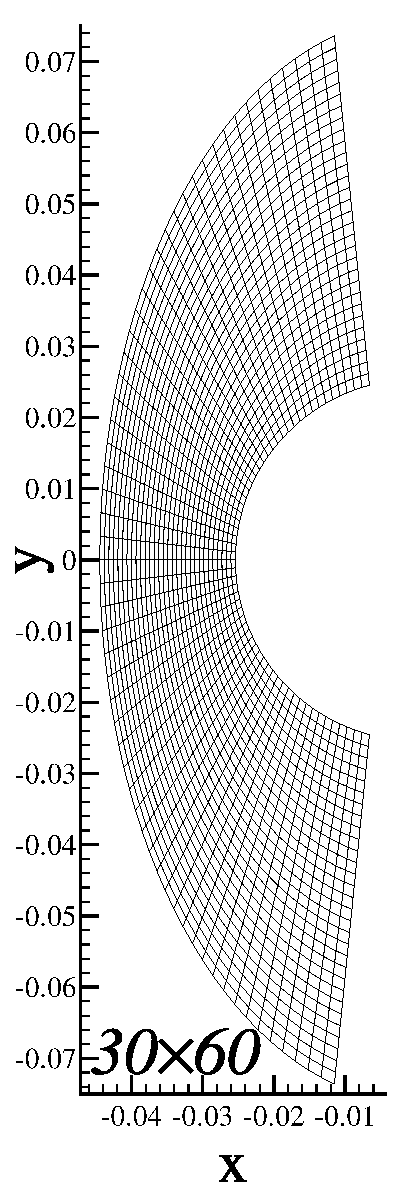
\includegraphics[height=0.5\textheight]{figures/hornung_N2_cylinder/mesh}
    \caption{Coarse computational grid for dissociating nitrogen flow over a cylinder\label{fig:hornung_cyl_n2_30x60}}
  \end{center}
\end{figure}

% This example is  a prototype for convection-dominated supersonic and hypersonic problems which arise in aerospace engineering.  The performance of the finite element algorithm presented in the previous sections will be examined in detail for this example.  The results of the numerical experiments performed in this section will be generalized and applied to more physically complicated flow phenomena in later application studies.

The simulation is initialized with uniform freestream values and marched in time until steady--state is reached.  A supersonic inflow boundary condition in which the conserved variables $\left[\rho_s, \rho u, \rho v, \rho E, \rho e_V\right]^T$ are specified as essential boundary conditions on the upstream inflow boundary. At the outflow boundary the flow is supersonic, and hence no outflow boundary conditions are specified for this inviscid flow.  The no--penetration boundary condition~$\bv{u}\cdot\nhat=0$ holds on the cylinder surface and is enforced as a natural boundary condition through the boundary integral in the weak statement as described in Reference~\citen{fins_ijnmf}.

 Figure~\ref{fig:hornung_cyl_flowfield} illustrates the steady-state flowfield for this case.  For this inviscid case the governing Euler equations are hyperbolic and admit discontinuous solutions. As expected, the cylinder produces a strong bow shock across which the density, velocity, and pressure jump. 
% Cylinder flow contours
\begin{figure}[hbtp]
  \begin{center}
    \subfigure[Pressure  \label{fig:hornung_cyl_pressure}]{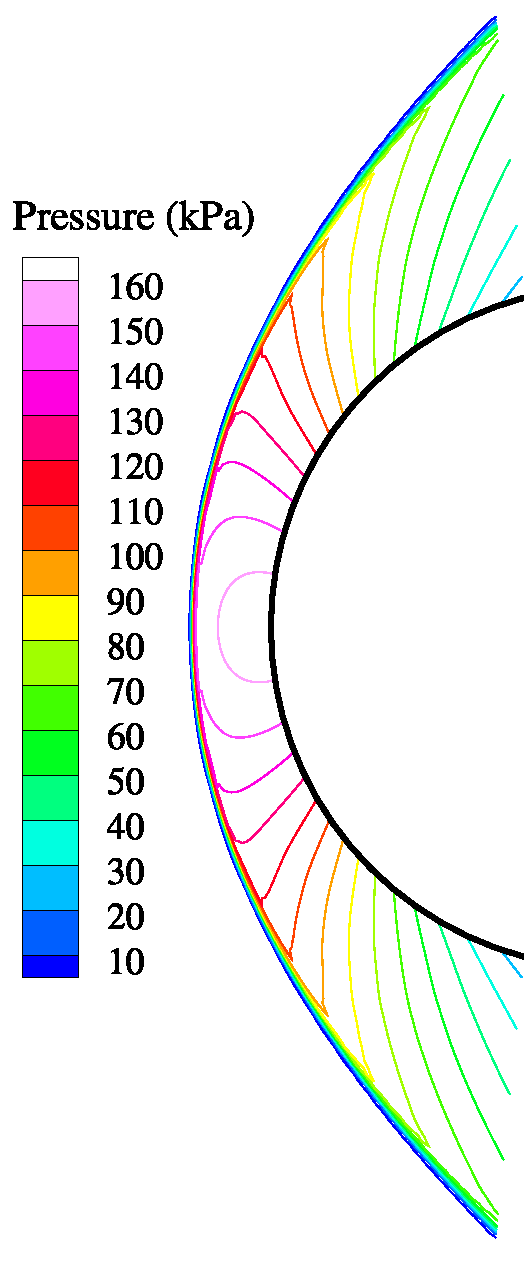
\includegraphics[width=0.22\textwidth]{figures/hornung_N2_cylinder/pressure}}
    \subfigure[Temperature  \label{fig:hornung_cyl_temp} ]{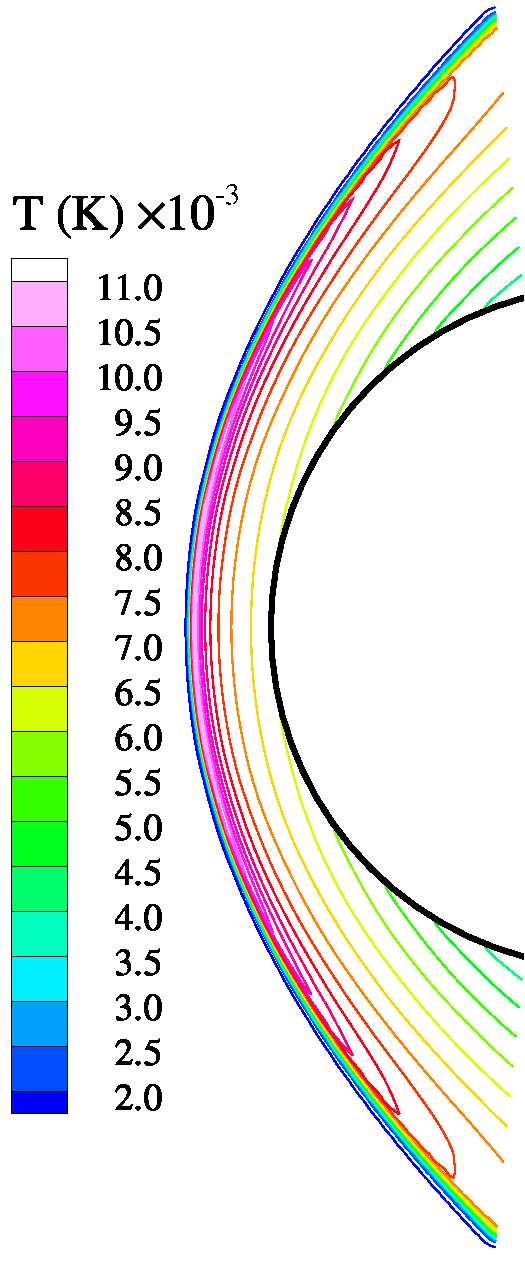
\includegraphics[width=0.22\textwidth]{figures/hornung_N2_cylinder/temperature}} 
    \subfigure[N$_2$ Concentration\label{fig:hornung_cyl_cN2}    ]{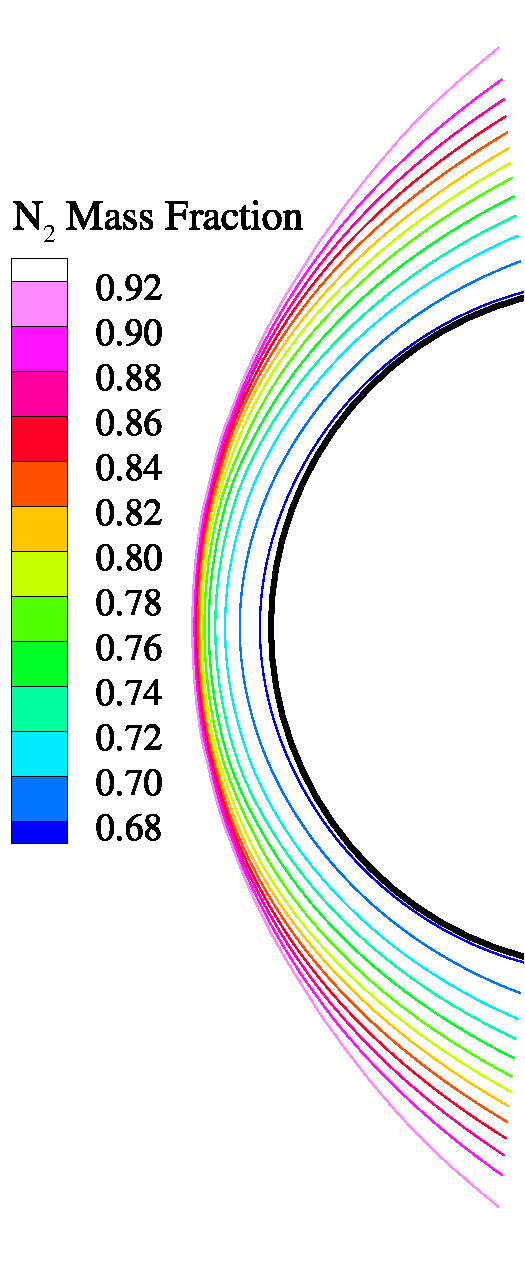
\includegraphics[width=0.22\textwidth]{figures/hornung_N2_cylinder/cN2}}
    \subfigure[N Concentration\label{fig:hornung_cyl_cN}     ]{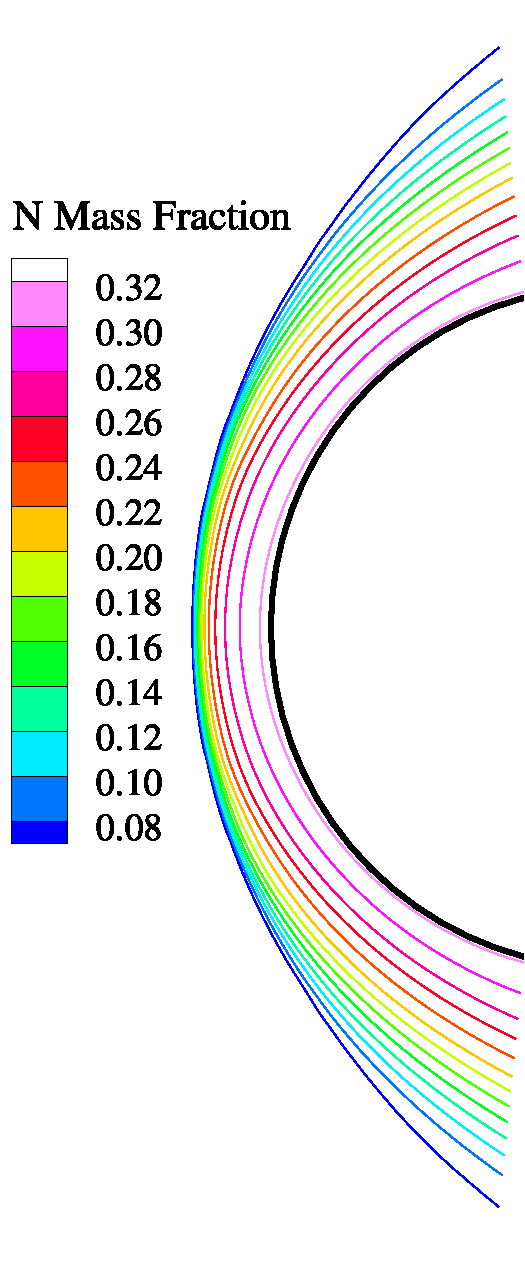
\includegraphics[width=0.22\textwidth]{figures/hornung_N2_cylinder/cN}} 
    \caption{Illustration of flowfield for dissociating nitrogen flow over a cylinder\label{fig:hornung_cyl_flowfield}}
  \end{center}
\end{figure}
Of particular interest is the static temperature field shown in Figure~\ref{fig:hornung_cyl_temp}, which is in sharp contrast to the typical calorically perfect gas result in which the post-shock stagnation region temperature is essentially constant.  In this reacting flow the gas reaches temperatures in excess of \unit[11,000]{K} immediately behind the shock wave.  At such extreme temperatures, however, N$_2$ becomes vibrationally excited and begins to dissoctate.  This is depicted in Figures~\ref{fig:hornung_cyl_cN2} and~\ref{fig:hornung_cyl_cN} by the decrease in N$_2$ and increase in N mass fractions, respectively.  (Since there are only two modeled in this case, the species distributions are essentially inverses of each other because of the requirement that everywhere c$_{\text{N}_2}+$c$_{\text{N}}=1$.)

The behavior for the specific case of the stagnation line is shown more quantitatively in Figure~\ref{fig:hornung_stag_line}, which shows the static temperature and mass fraction distributions along the stagnation line.
\begin{figure}
  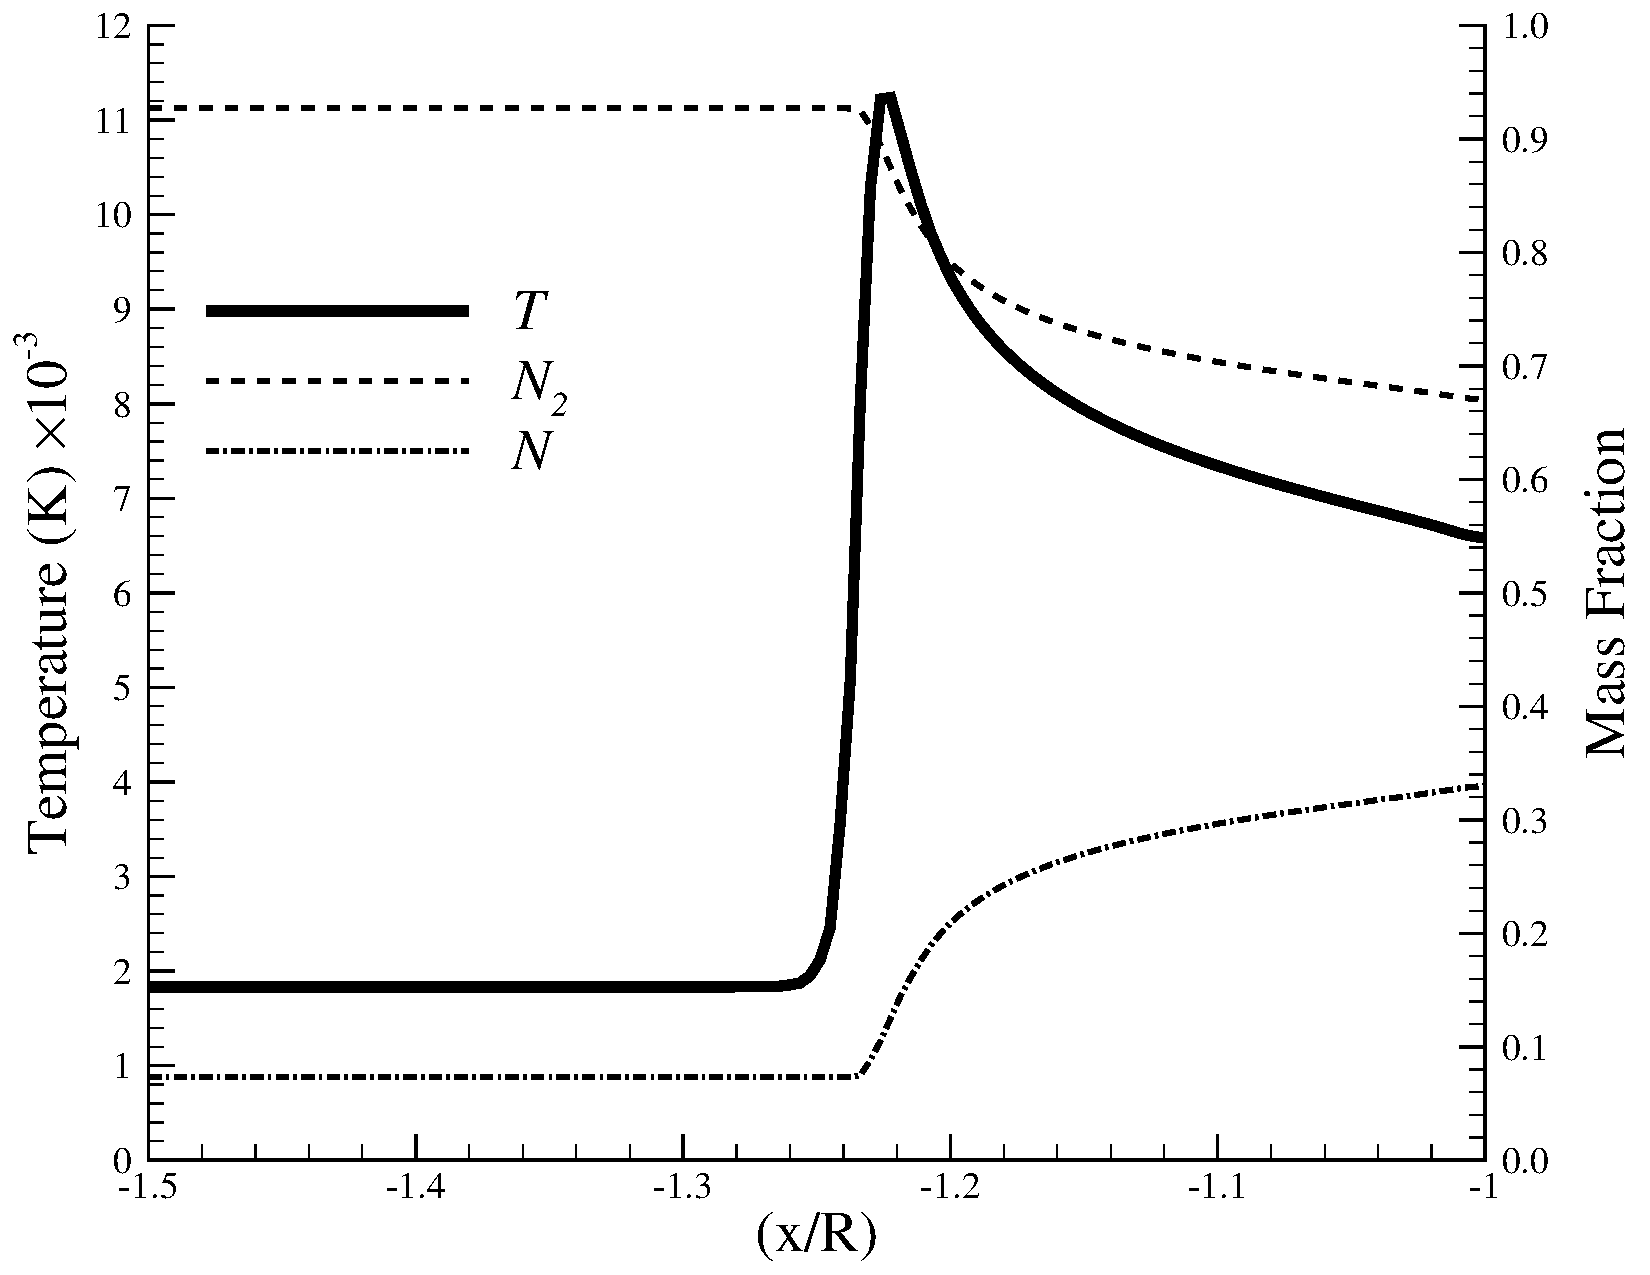
\includegraphics[width=\textwidth]{figures/hornung_N2_cylinder/stagline}
  \caption{Stagnation line temperature and species mass fractions for inviscid dissociating flow about a cylinder.\label{fig:hornung_stag_line}}
\end{figure}

The important question of mesh convergence is examined in Figure~\ref{fig:hornung_stagline_mesh_conv}, which depicts static pressure and temperature along the stagnation line for a family of meshes.  The coarsest mesh considered, $30\times 60$ elements, is clearly too coarse for this problem, underpredicting the pressure and overpredicting the temperature in the shock layer.
% stagnation line mesh convergence
\begin{figure}[hbtp]
  \begin{center}
    \subfigure[Pressure  \label{fig:hornung_stagline_mesh_conv_pressure}]{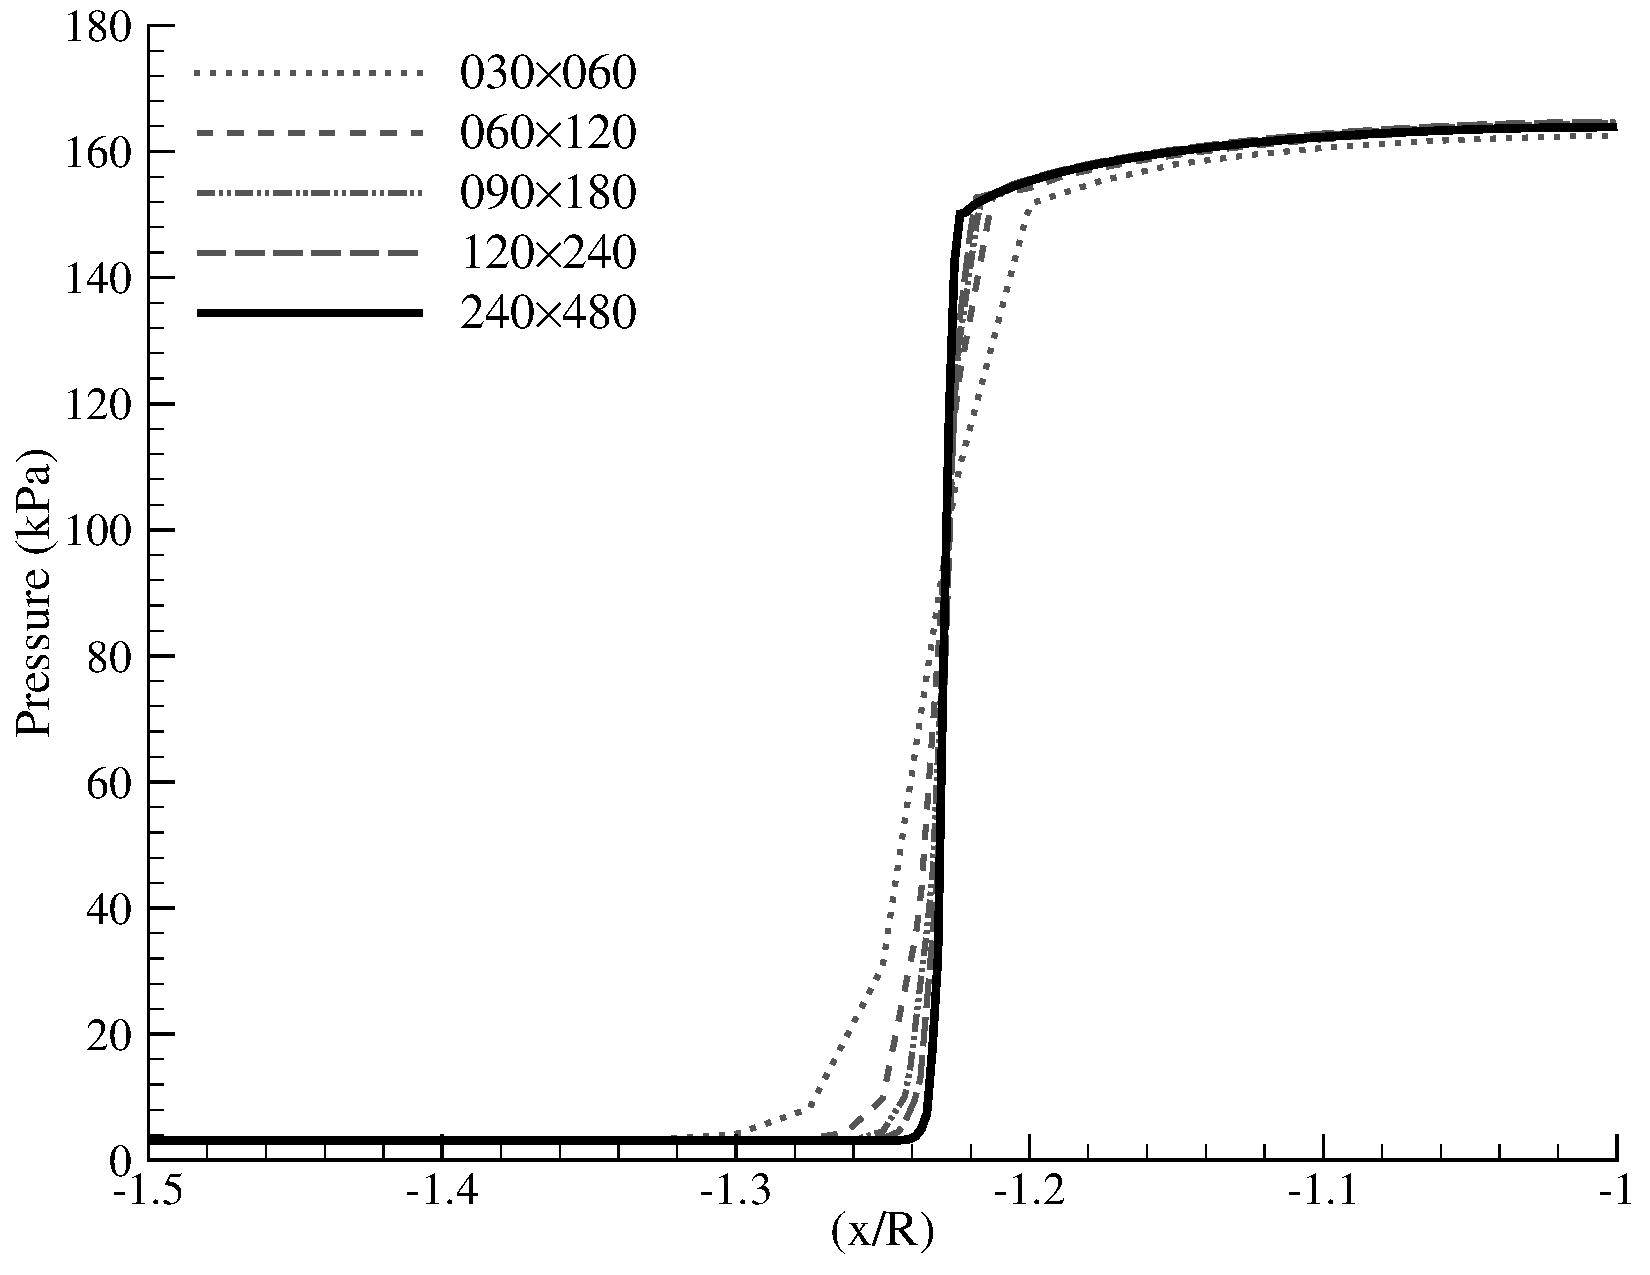
\includegraphics[width=0.48\textwidth]{figures/hornung_N2_cylinder/stagline_mesh_conv_P}}
    \subfigure[Temperature  \label{fig:hornung_stagline_mesh_conv_temperature} ]{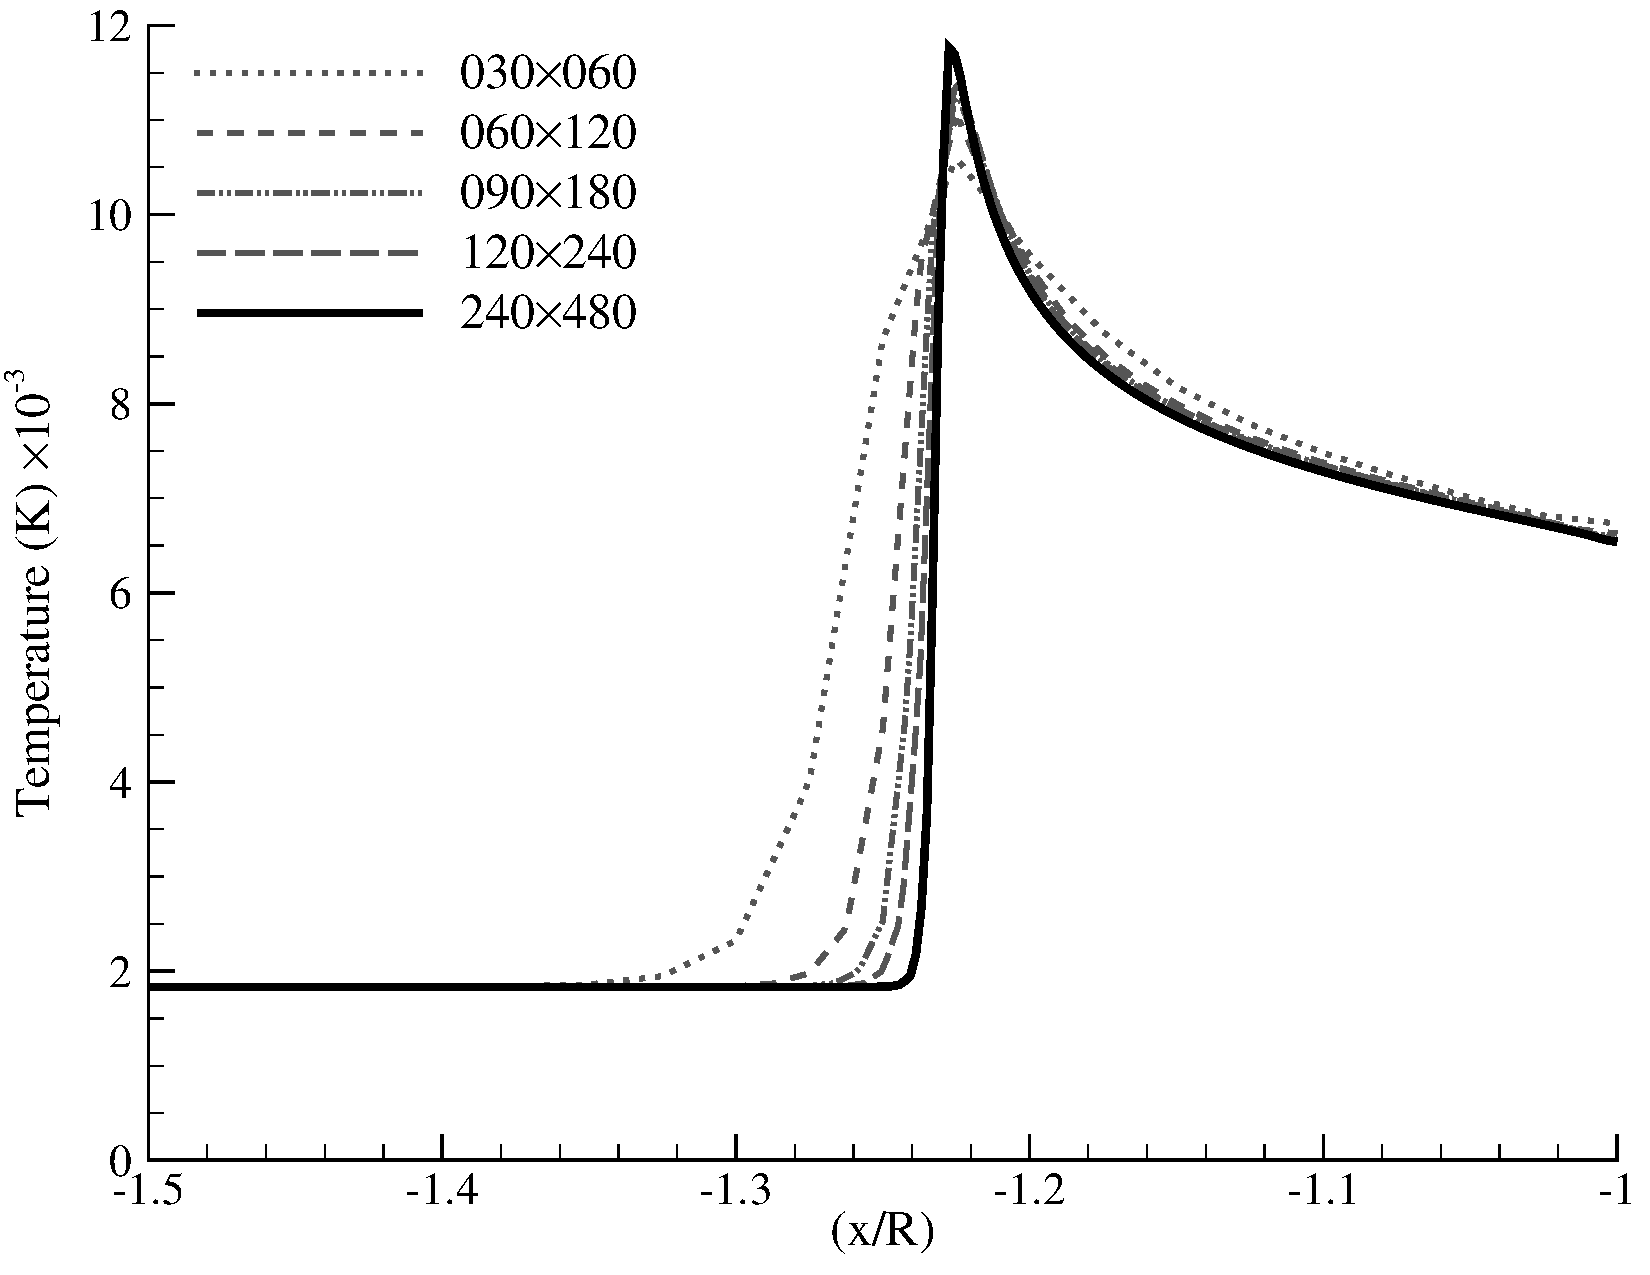
\includegraphics[width=0.48\textwidth]{figures/hornung_N2_cylinder/stagline_mesh_conv_T}} 
    \caption{Stagnation line property mesh convergence for dissociating nitrogen flow over a cylinder\label{fig:hornung_stagline_mesh_conv}}
  \end{center}
\end{figure}
It is clear from this coarse mesh, however, that the shock is captured approximately over 3--4 elements.  This trend is repeated for all finer meshes.  The discrete shockwave is self-similar in this regard because of the lack of physical diffusion in this problem -- its thickness is determined solely by the local mesh spacing.

\begin{figure}
  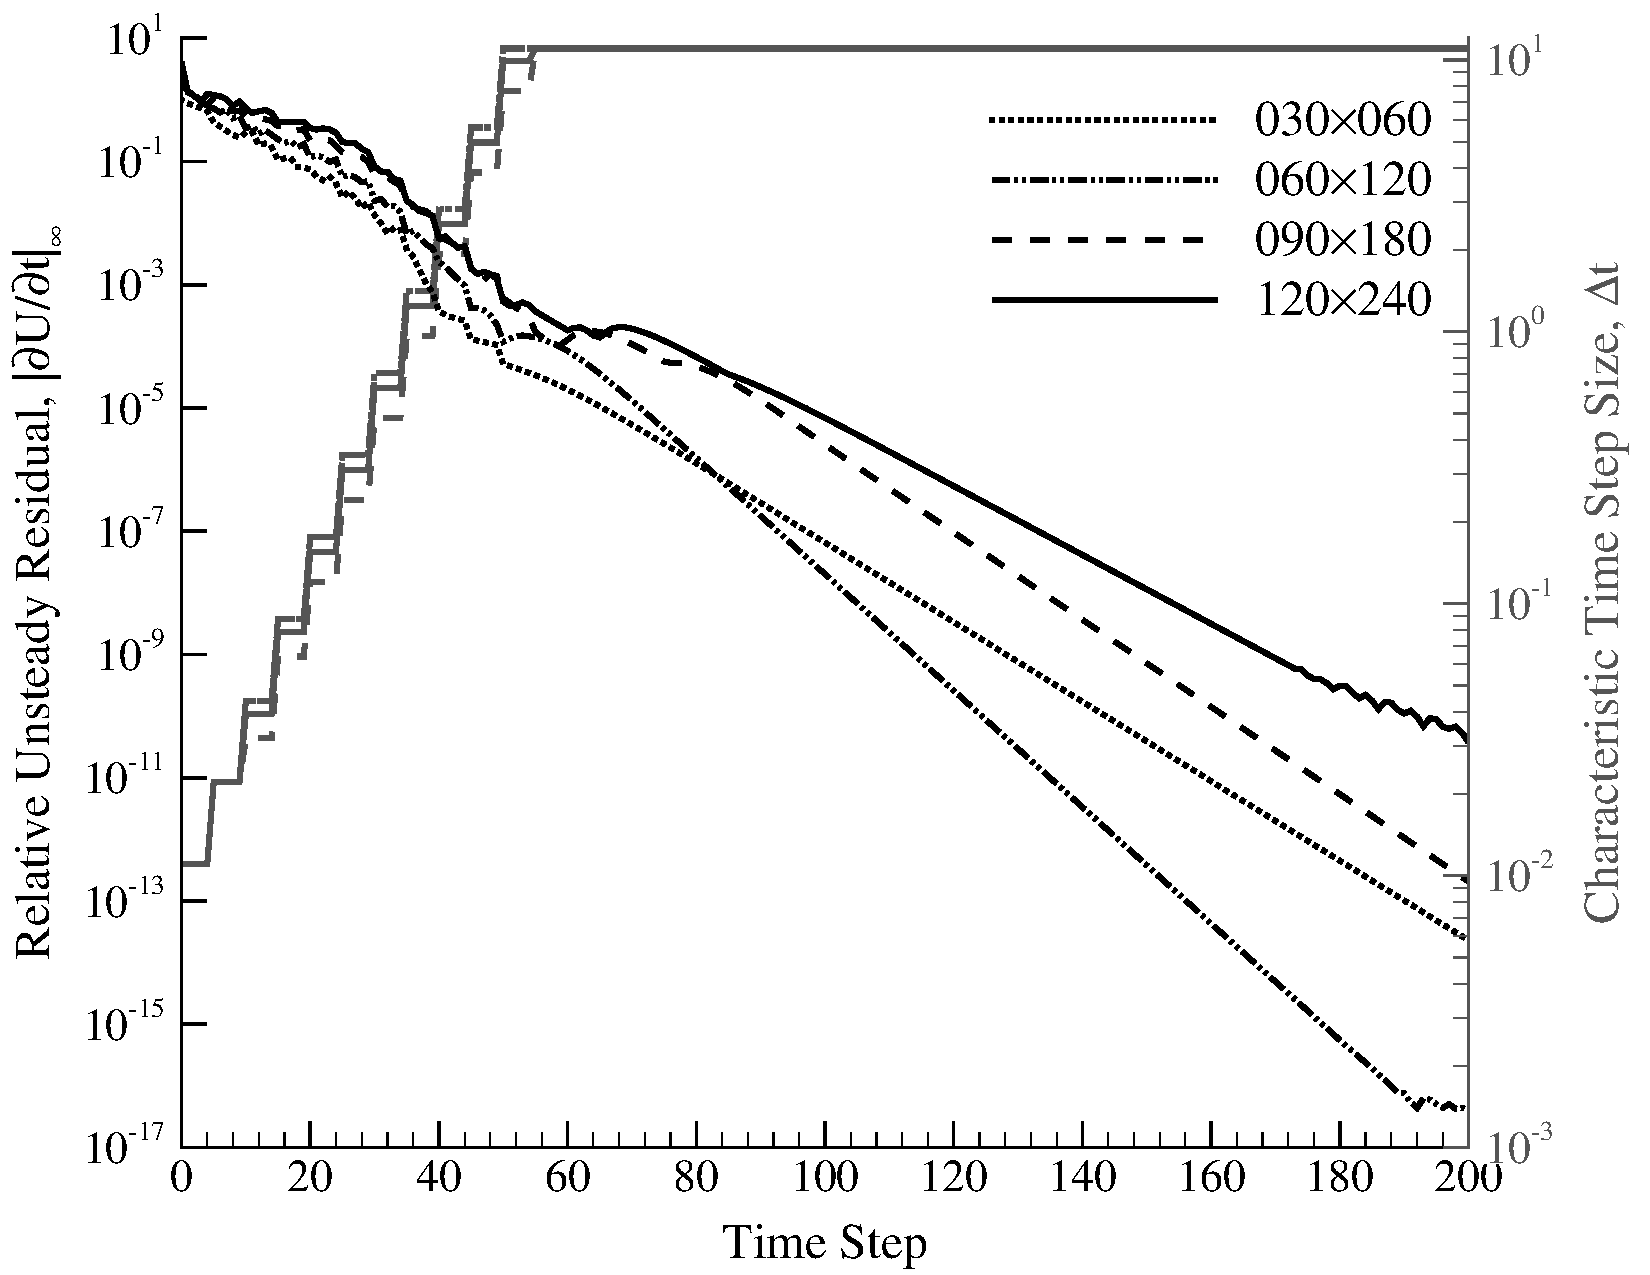
\includegraphics[width=\textwidth]{figures/hornung_N2_cylinder/conv}
  \caption{Transient convergence for inviscid dissociating nitrogen flow about a cylinder.\label{fig:hornung_conv}}
\end{figure}


\begin{figure}
  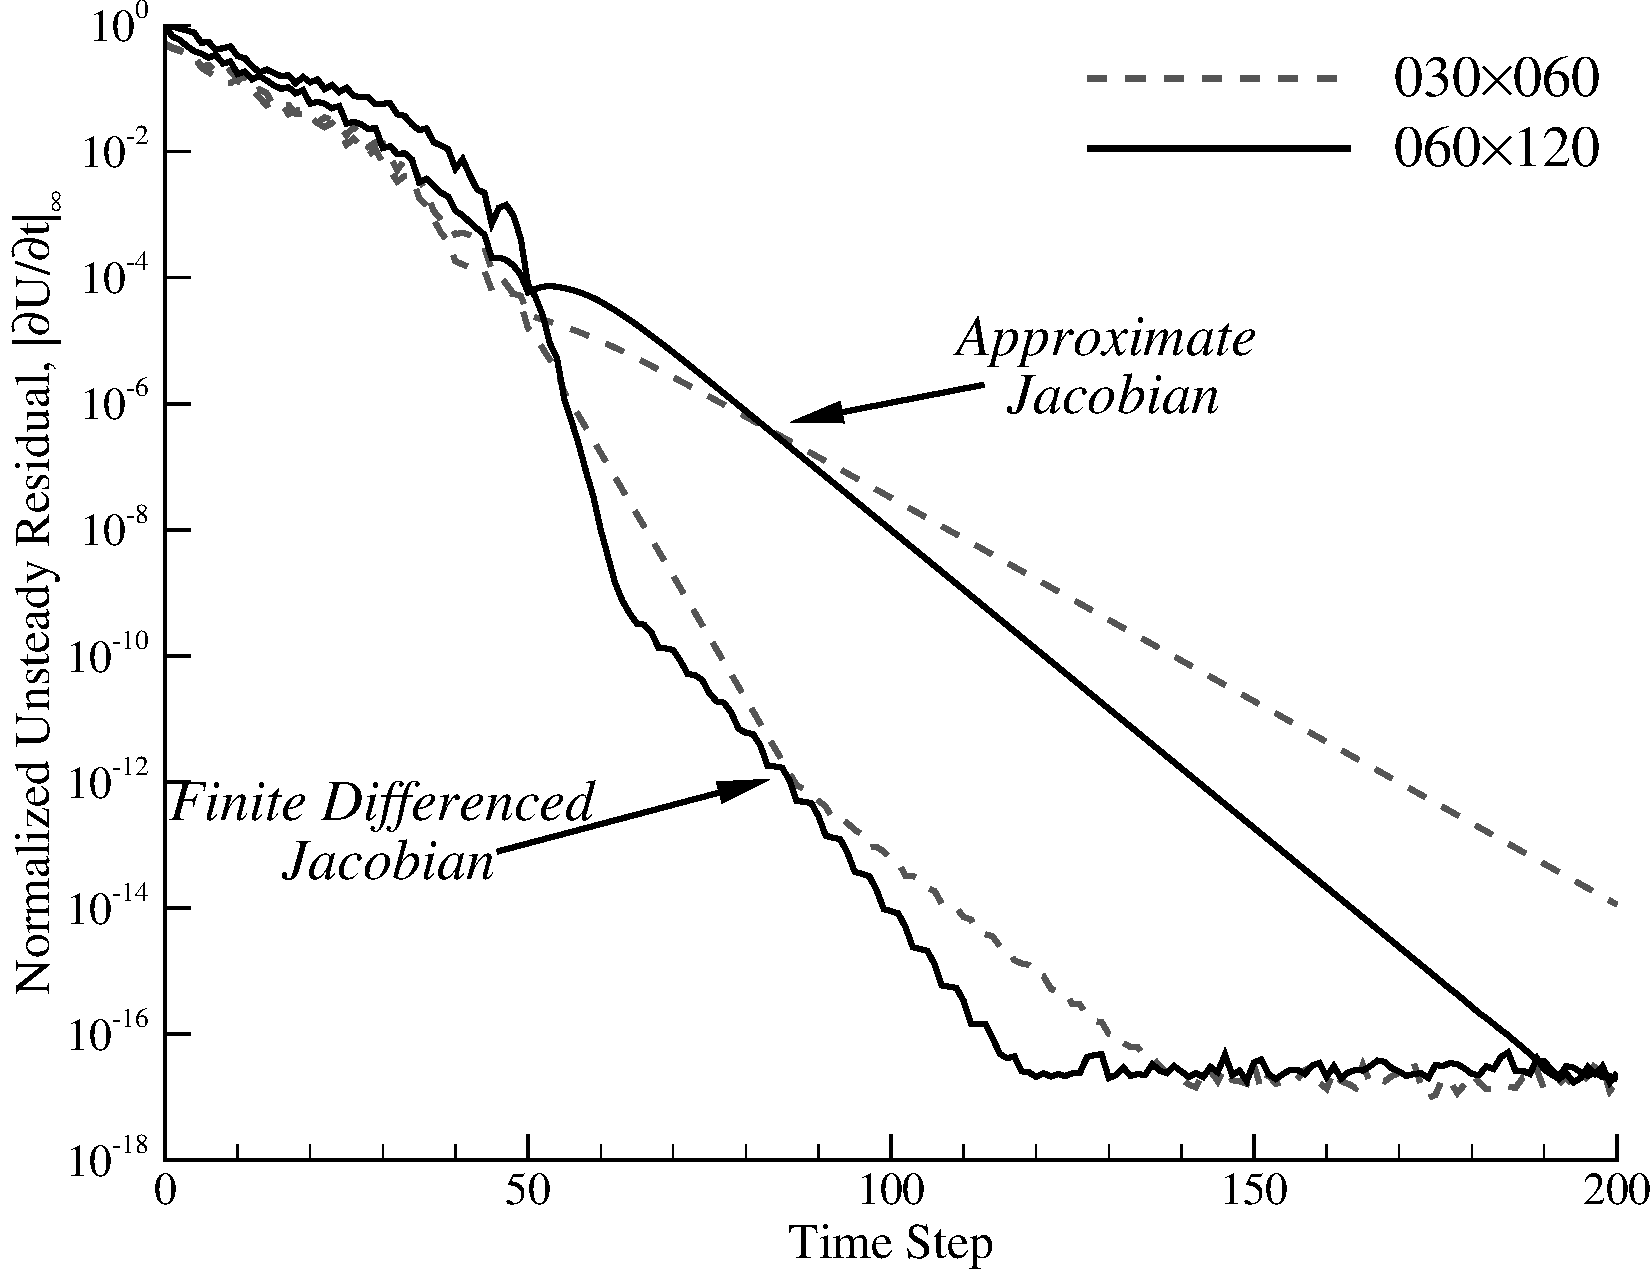
\includegraphics[width=\textwidth]{figures/hornung_N2_cylinder/approx_vs_fd_jacobian}
  \caption{Influence of linearization strategy for inviscid dissociating nitrogen flow about a cylinder.\label{fig:hornung_jac_comp_conv}}
\end{figure}



%%%%%%%%%%%%%%%%%%%%%%%%%%%%%%%%%%%%%%%%%%%%%%%%%%%%%%%%%%%%%%%%%%%%%%%%%%%%%%%
\subsection{Dissociating Air Flow Over A Cylinder\label{sec:comp_ns_cyl_air}}
A second inviscid case considers dissociating air flow about a cylinder.  In this case the reacting gas model contains the five species N$_2$, O$_2$, NO, N, and O. The freestream mass fractions of N$_2$ and O$_2$ are 0.78 and 0.22, respectively.
% Cylinder flow contours
\begin{figure}[hbtp]
  \begin{center}
    \subfigure[Pressure  \label{fig:5sp_air_cyl_pressure}]{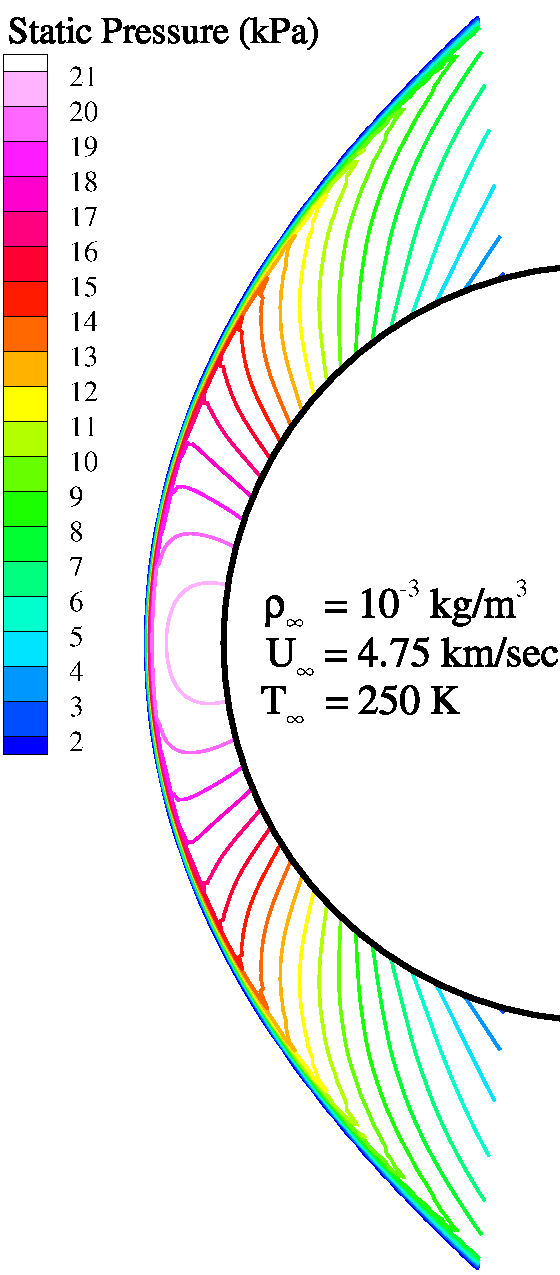
\includegraphics[width=0.3\textwidth]{figures/cyl_5sp_air/fins_P}}
    \subfigure[Temperature  \label{fig:5sp_air_cyl_temp} ]{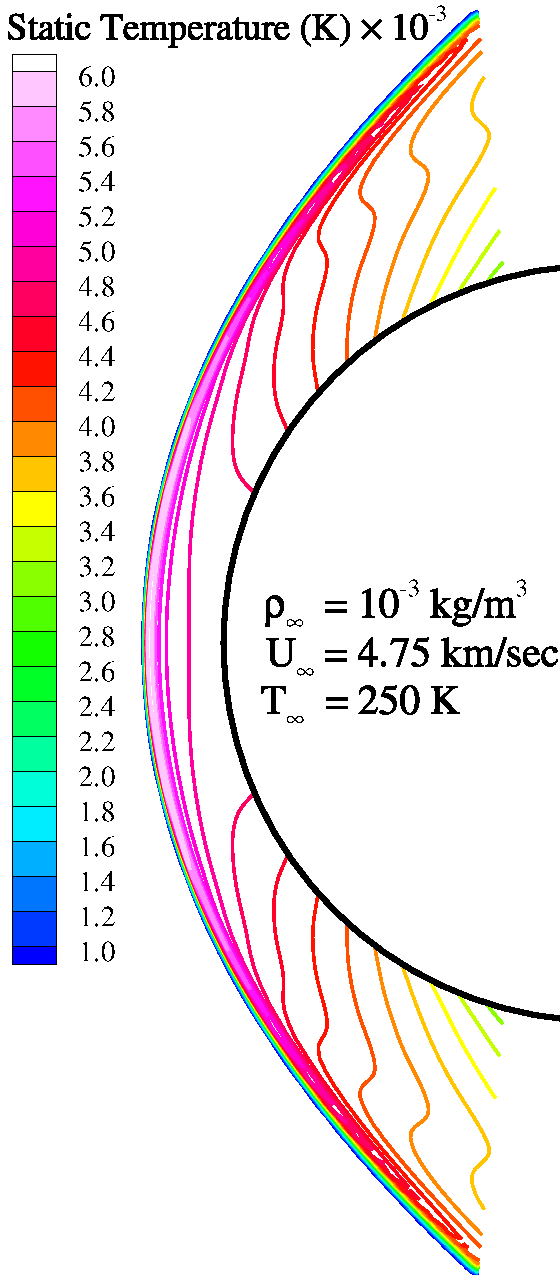
\includegraphics[width=0.3\textwidth]{figures/cyl_5sp_air/fins_T}}
    \caption{Illustration of flowfield for dissociating air flow over a cylinder\label{fig:5sp_air_cyl_flowfield}}
  \end{center}
\end{figure}
The freestream is characterized by density, velocity, and temperature, whose values are $\rho_\infty=\unitfrac[10^{-3}]{kg}{m^3}$, $u_\infty=\unitfrac[4.75]{km}{sec}$, and $T_\infty=\unit[250]{K}$.
% Cylinder flow contours
\begin{figure}[hbtp]
  \begin{center}
    \subfigure[N$_2$ Concentration]{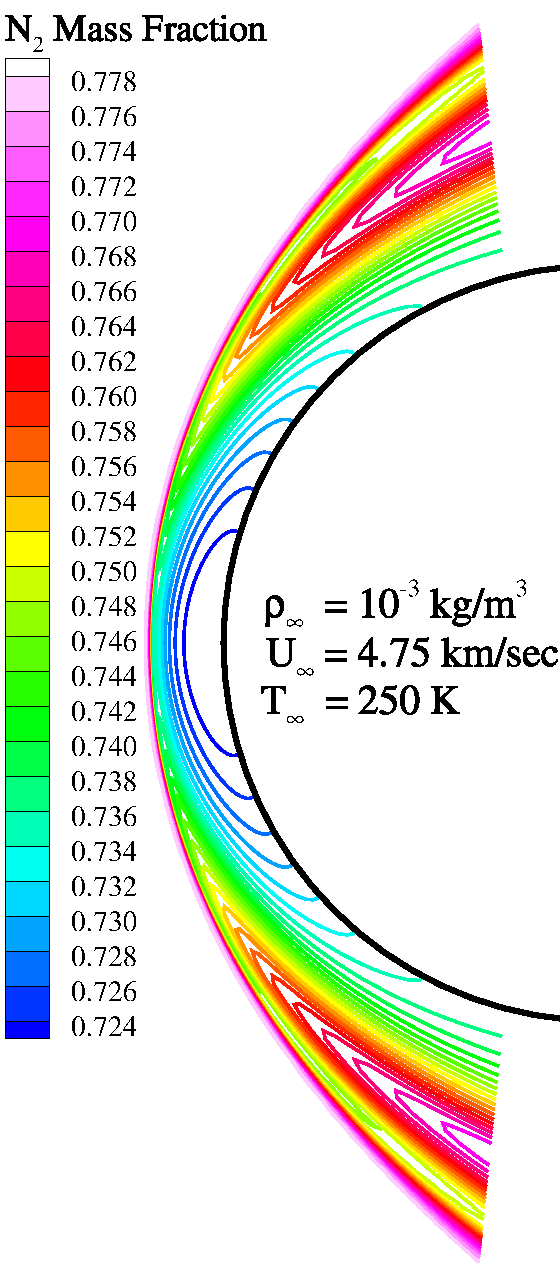
\includegraphics[width=0.3\textwidth]{figures/cyl_5sp_air/fins_cN2}}
    \subfigure[O$_2$ Concentration]{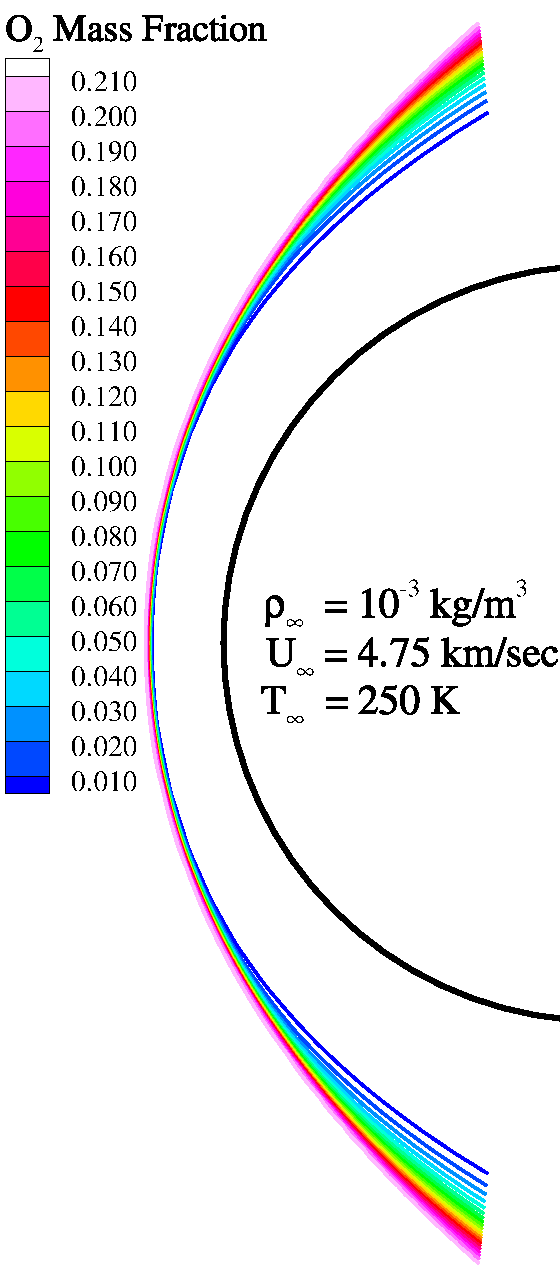
\includegraphics[width=0.3\textwidth]{figures/cyl_5sp_air/fins_cO2}}
    \subfigure[NO Concentration]{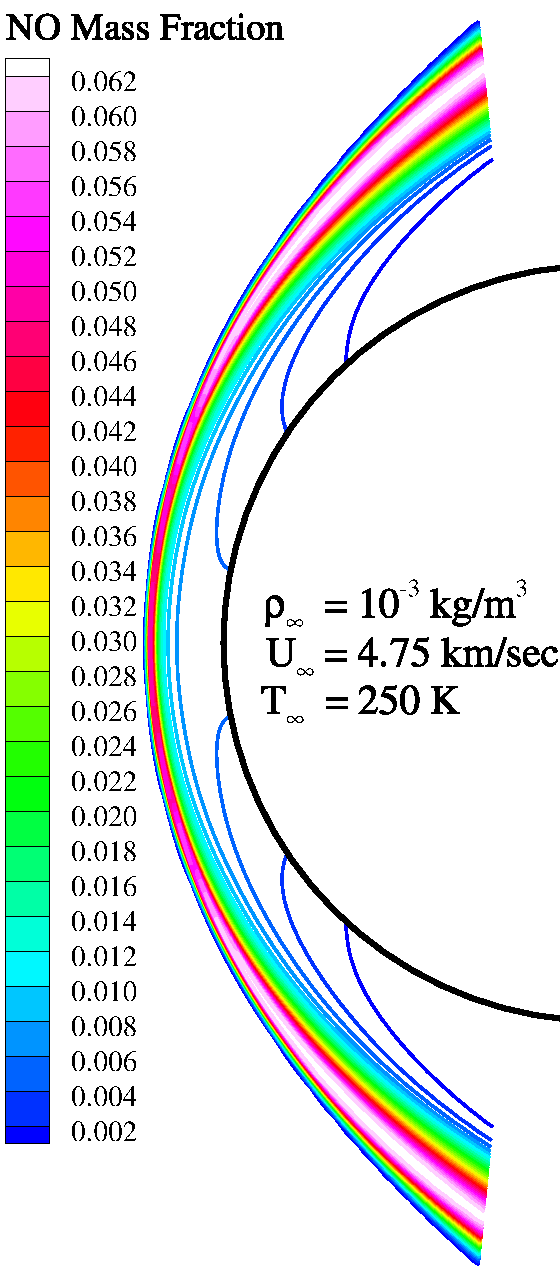
\includegraphics[width=0.3\textwidth]{figures/cyl_5sp_air/fins_cNO}} \\
    \subfigure[N Concentration]{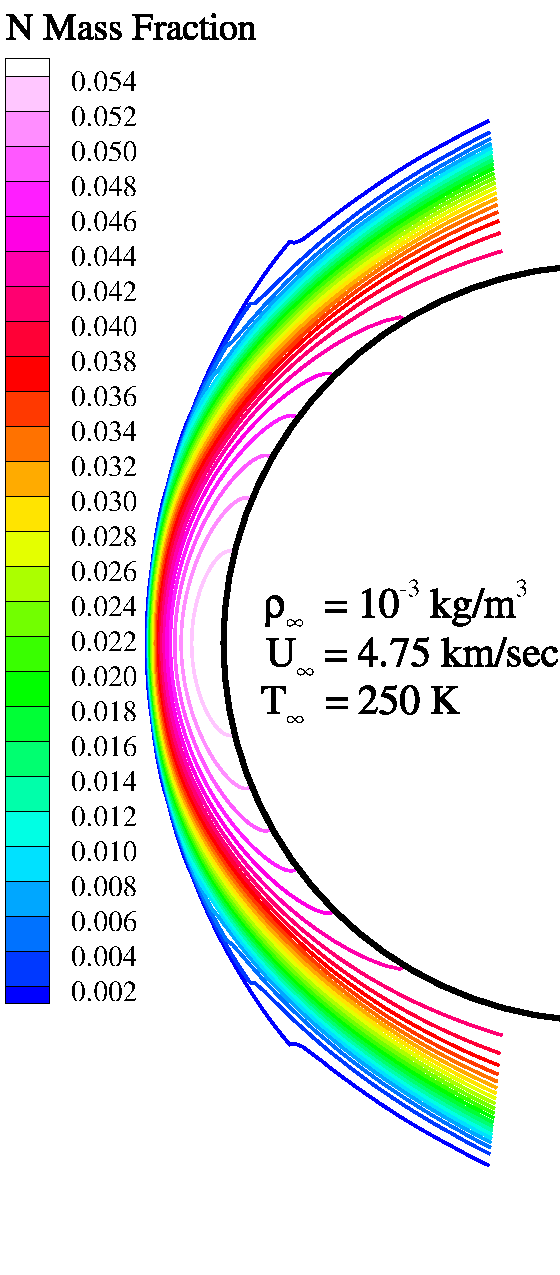
\includegraphics[width=0.3\textwidth]{figures/cyl_5sp_air/fins_cN}}
    \subfigure[O Concentration]{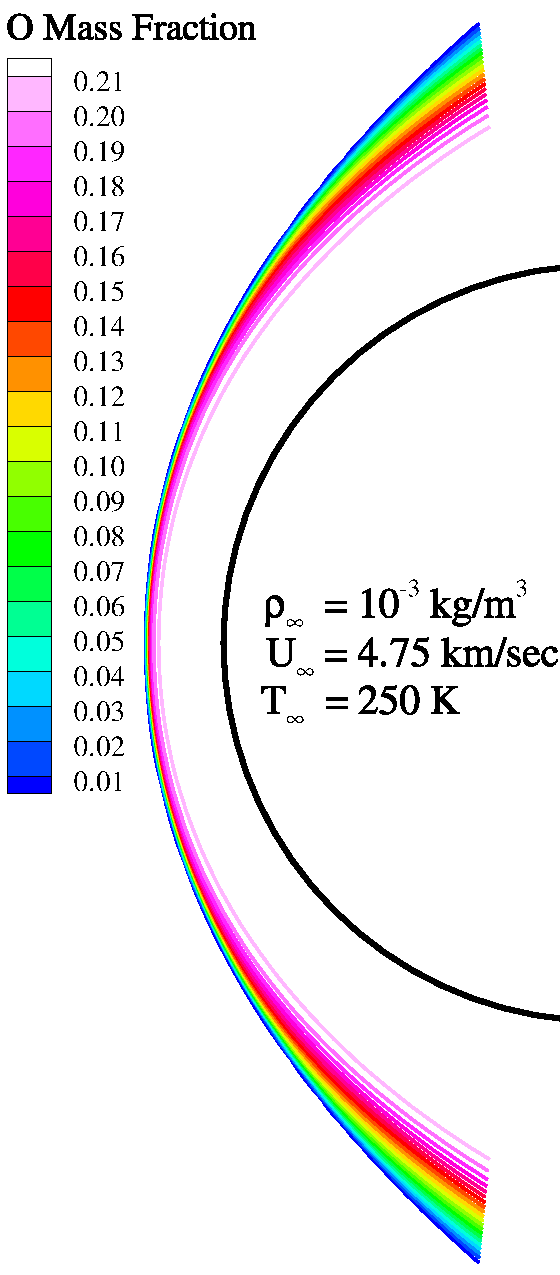
\includegraphics[width=0.3\textwidth]{figures/cyl_5sp_air/fins_cO}}
    \caption{Illustration of flowfield for dissociating air flow over a cylinder: molecular species\label{fig:5sp_air_cyl_flowfield_concentrations_molecules}}
  \end{center}
\end{figure}


\begin{figure}[hbtp]
  \begin{center}
    \subfigure[Pressure]{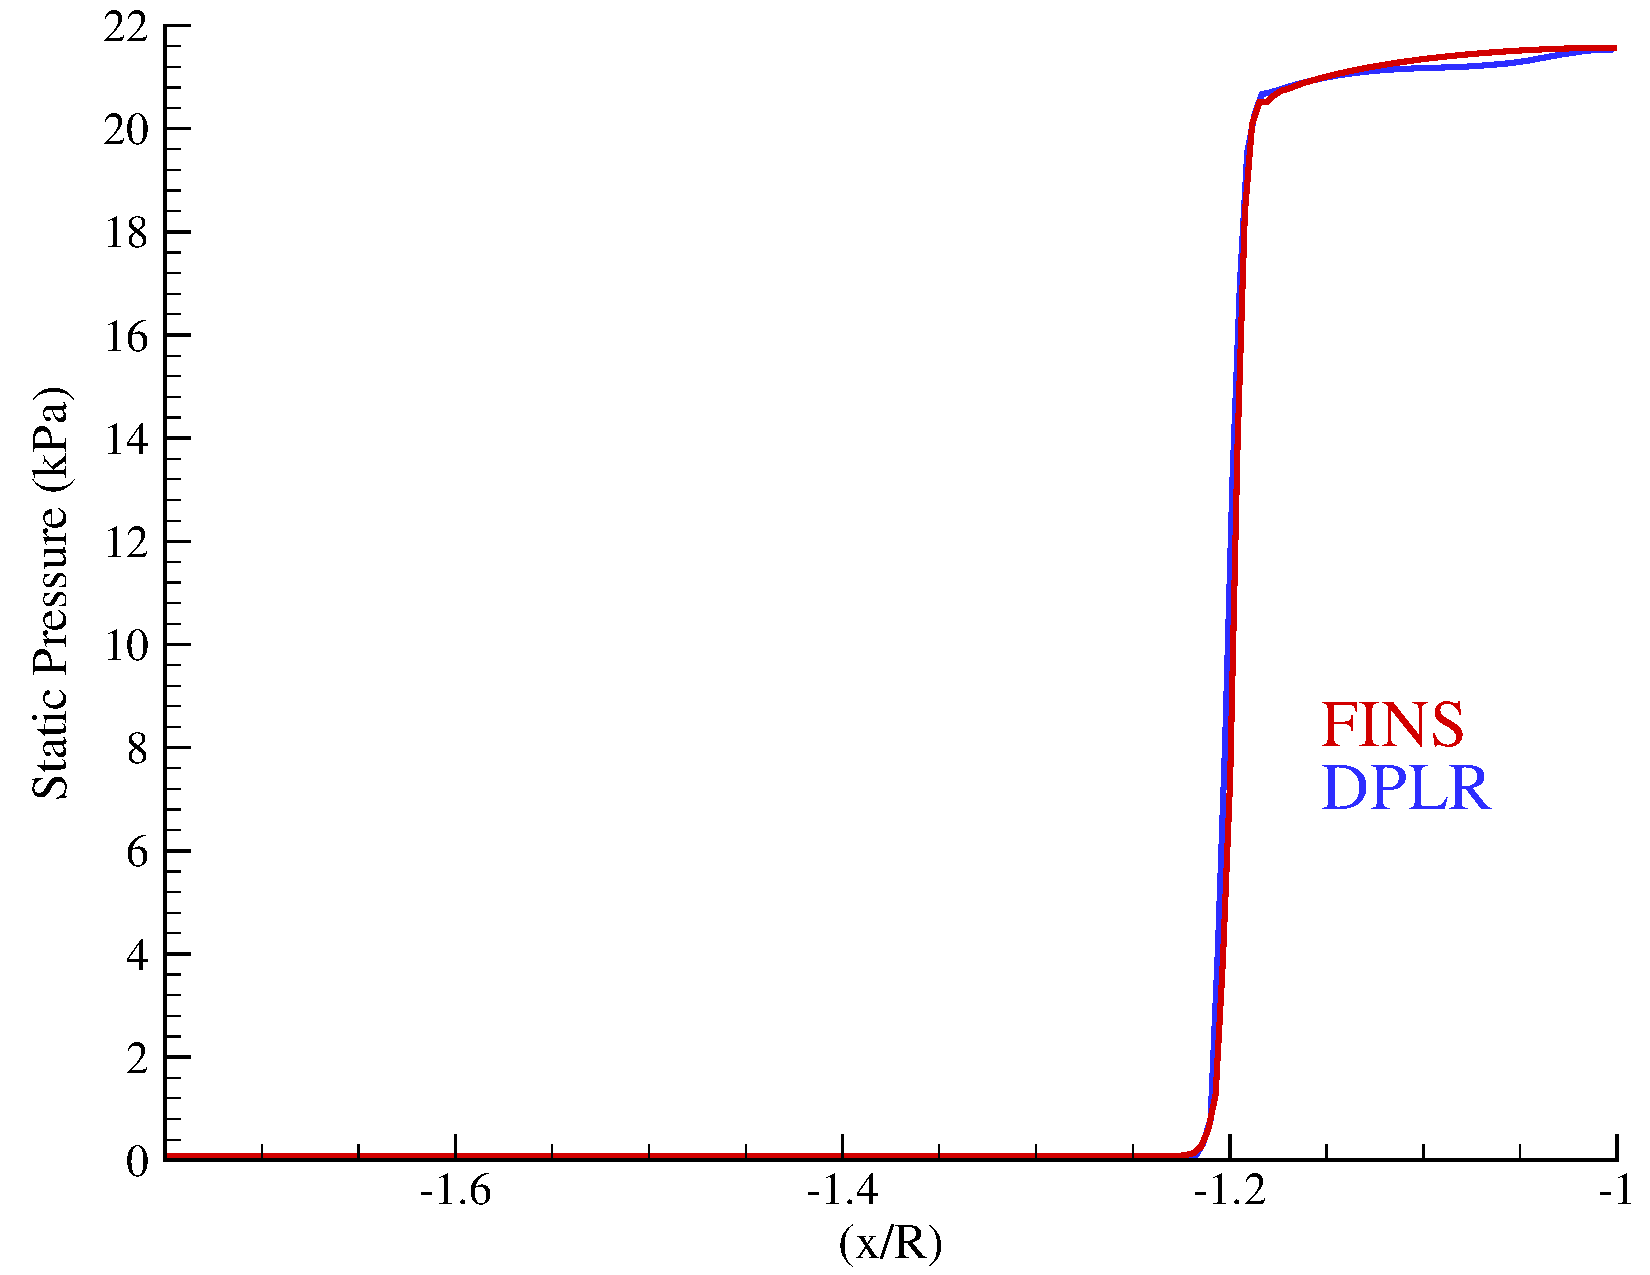
\includegraphics[width=0.48\textwidth]{figures/cyl_5sp_air/fins_dplr_P_comp}}
    \subfigure[Temperature]{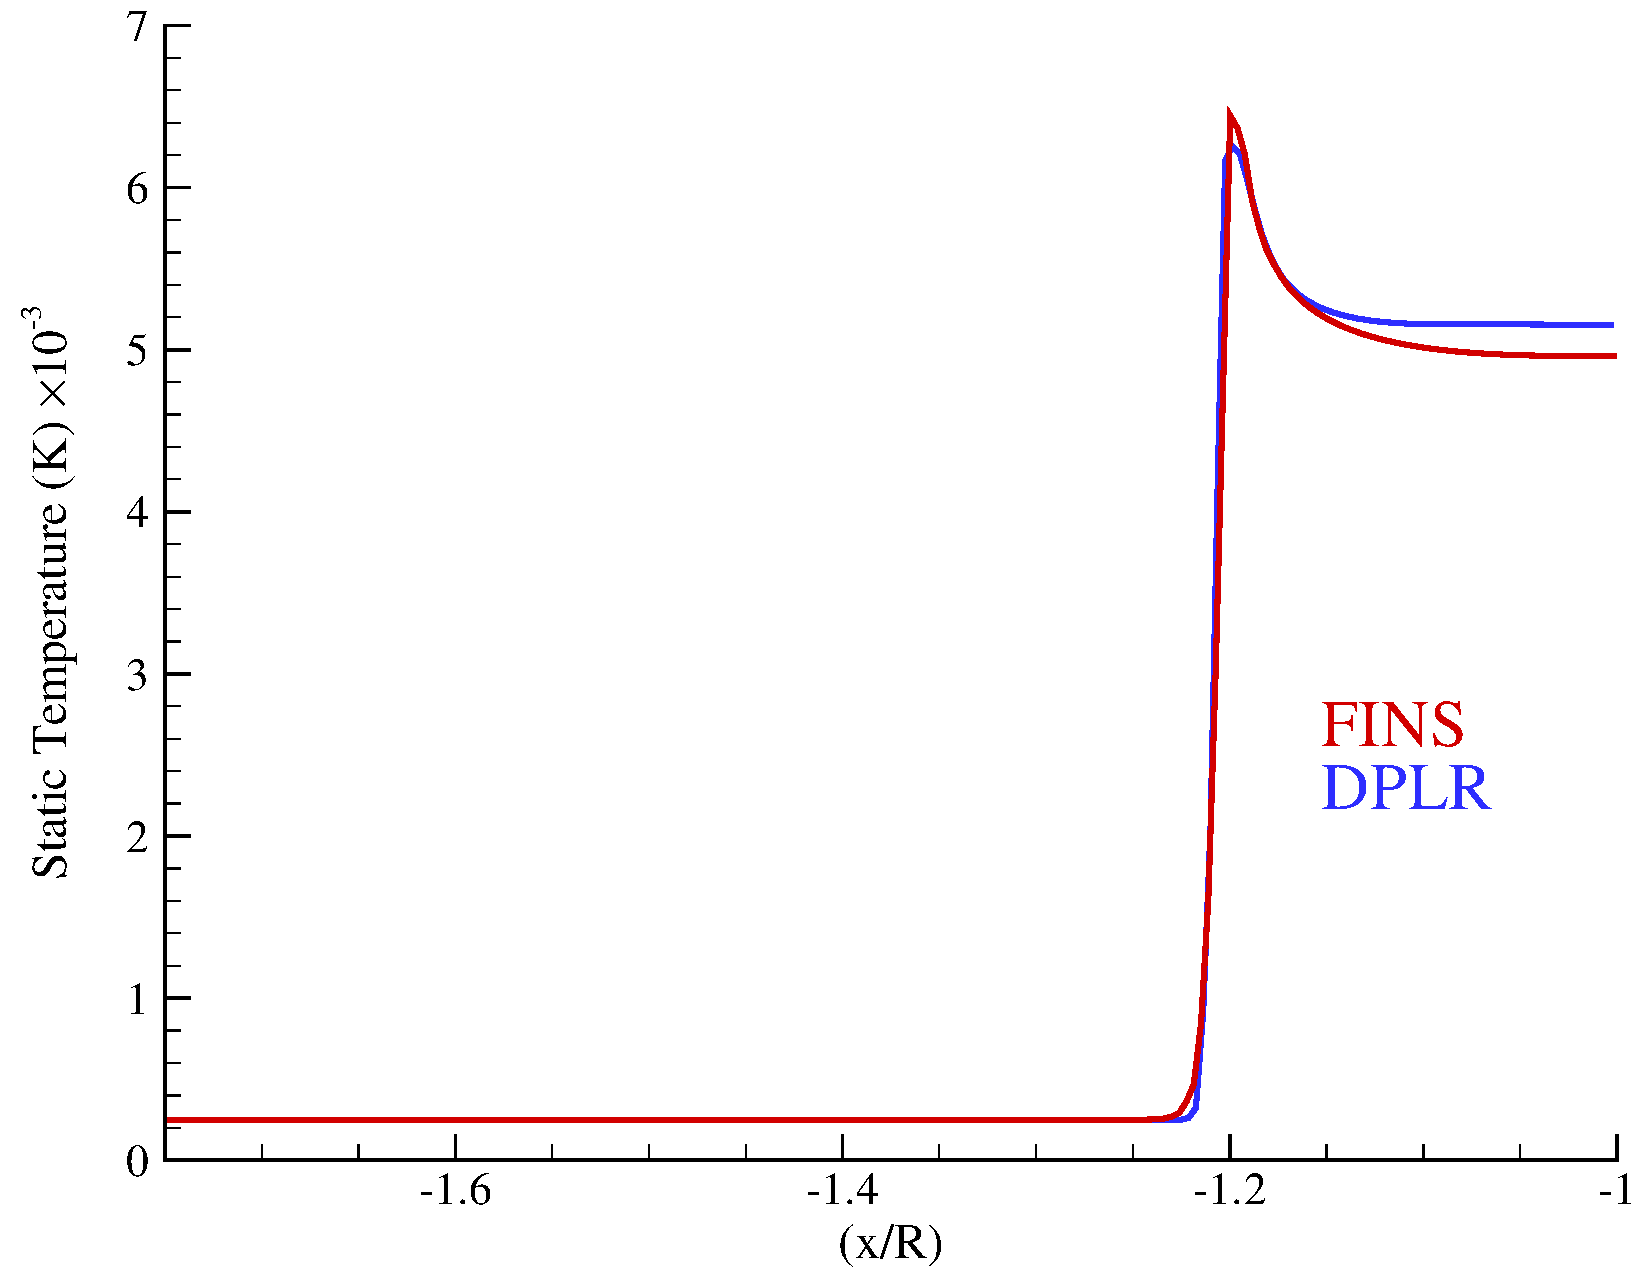
\includegraphics[width=0.48\textwidth]{figures/cyl_5sp_air/fins_dplr_T_comp}}
    \caption{Code-to-code comparison for dissociating air flow over a cylinder -- stagnation line pressure and temperature}
  \end{center}
\end{figure}


\begin{figure}[hbtp]
  \begin{center}
    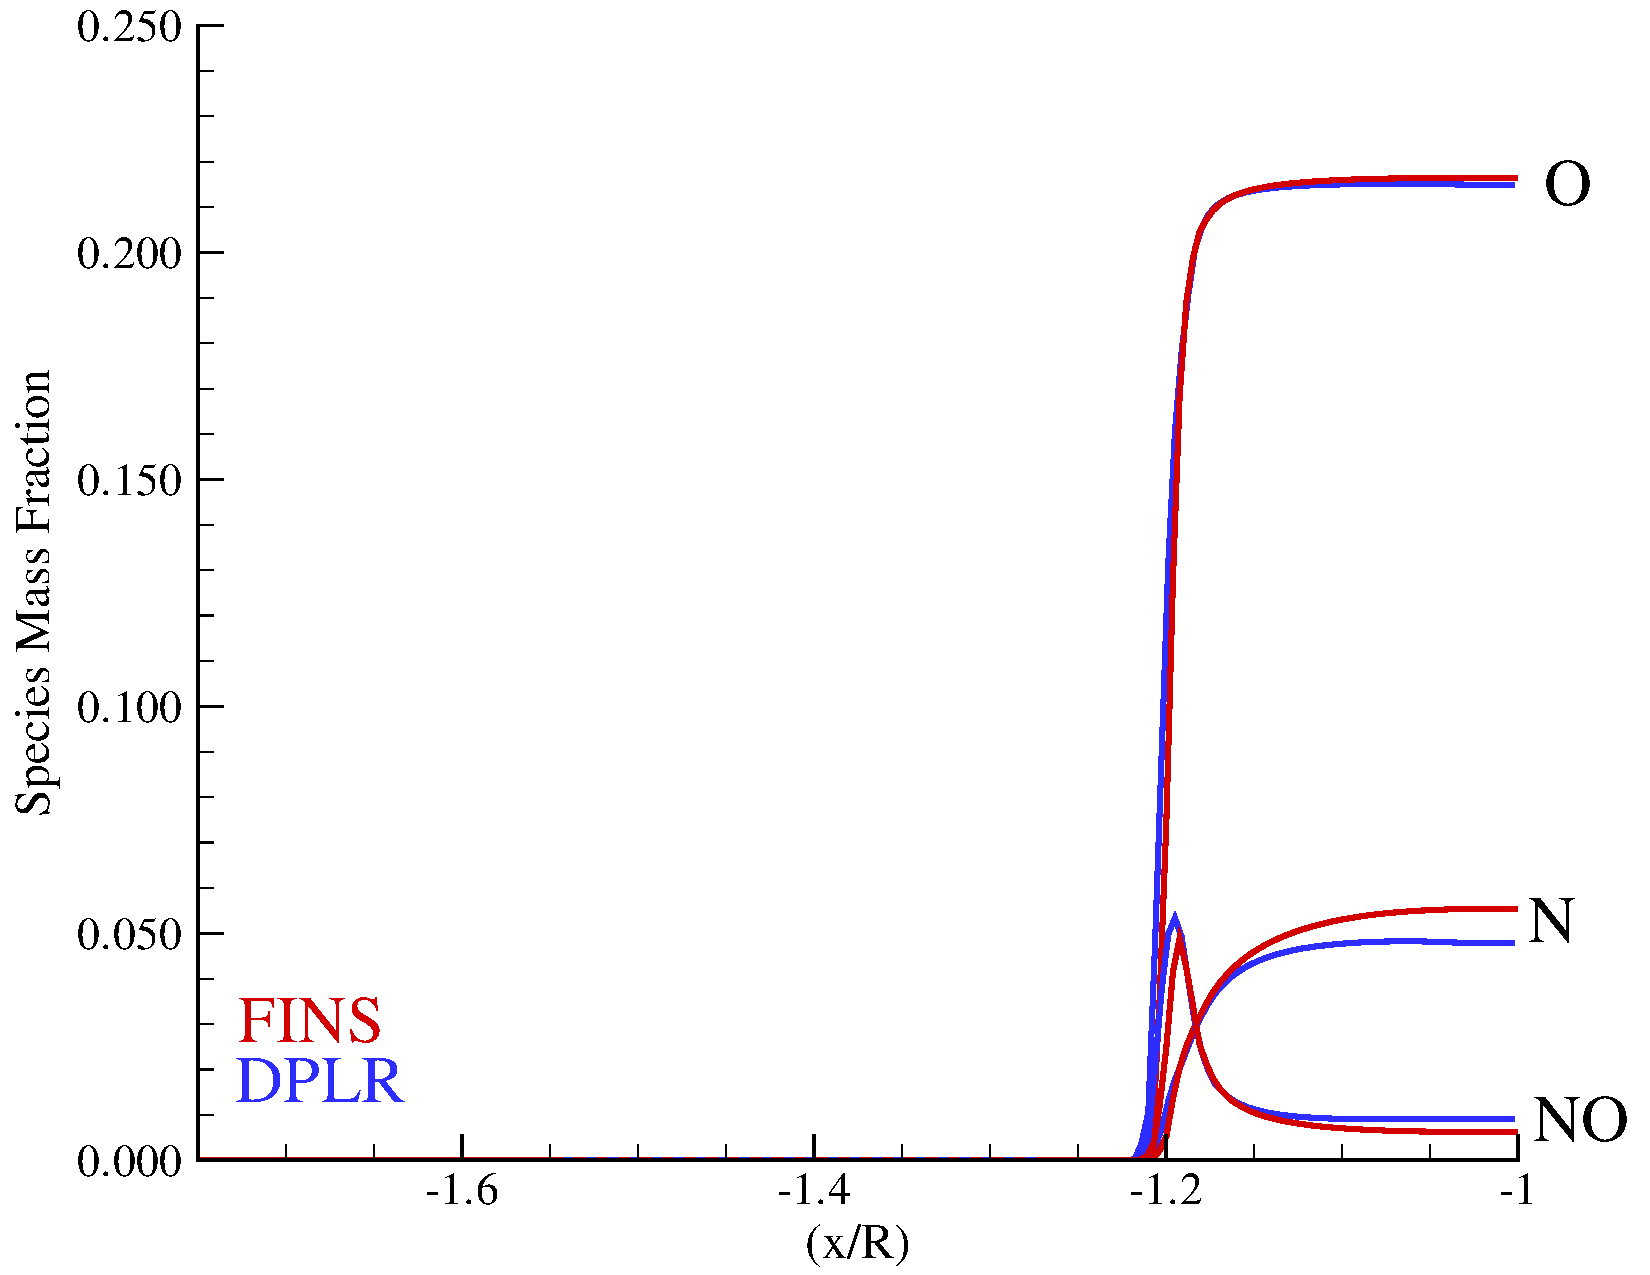
\includegraphics[width=\textwidth]{figures/cyl_5sp_air/fins_dplr_massfracs_comp}
    \caption{Code-to-code comparison for dissociating air flow over a cylinder -- species mass fractions}
  \end{center}
\end{figure}




%%%%%%%%%%%%%%%%%%%%%%%%%%%%%%%%%%%%%%%%%%%%%%%%%%%%%%%%%%%%%%%%%%%%%%%%%%%%%%%
\clearpage
\bibliography{paper}
\bibliographystyle{unsrt}


% LocalWords:  Navier EG Petrov Galerkin SUPG discretization nd discretizations
% LocalWords:  axisymmetric flowfields nondimensionalization eq pde sutherland
% LocalWords:  Prandtl nondimensionalized scalingx scalingmu nondimensional th
% LocalWords:  ik ij Jacobian jacobian discretized Wendroff nonequilibrium et
% LocalWords:  al Shakib Aliabadi diag NN el LeBeau Tezduyar upwinding TVD fe
% LocalWords:  aerothermodynamic freestream discretizing Hauke ungrouped Awruch
% LocalWords:  nodally Kessler priori Lobatto conv Courant Friedrichs Lewy CFL
% LocalWords:  Krylov linearization METIS subdomains decompostion subdomain un
% LocalWords:  semidiscrete udot unm euler ccc flowfield linsolve sys PETSc ILU
% LocalWords:  preconditioner mf nonlinearities GMRES Hugoniot subiterations ss
% LocalWords:  pre subproblem Catabriga Coutinho superlinearly Calspan CUBRC ns
% LocalWords:  calorically discretize streamwise centerline Lillard Peraire mol
% LocalWords:  libMeshPaper differenced Gnoffo equilibrate Fick's vib elec br
% LocalWords:  sr
